\documentclass[11pt,oneside]{article}
\usepackage[T1]{fontenc}
\usepackage[utf8]{inputenc}
\usepackage{lmodern}
\usepackage[margin=1in,headheight=15pt]{geometry}
\usepackage{amsmath,amssymb,amsthm,mathtools}
\usepackage{microtype,booktabs,longtable,array,enumitem}
\usepackage{graphicx,xcolor,listings,xurl,hyperref,fancyhdr}
\hypersetup{colorlinks=true,linkcolor=blue!45!black,citecolor=blue!45!black,urlcolor=blue!55!black,pdftitle={Continuous mathematics in iPRA: shared error budgets, integration, and stable homotopies},pdfauthor={Research report prepared for Vladimir Reshetnikov}}
\setlength{\emergencystretch}{3em}
\setlist{itemsep=3pt,topsep=5pt,leftmargin=*}
\newcolumntype{P}[1]{>{\raggedright\arraybackslash}p{#1}}
\newtheorem{theorem}{Theorem}[section]
\newtheorem{lemma}[theorem]{Lemma}
\newtheorem{proposition}[theorem]{Proposition}
\newtheorem{corollary}[theorem]{Corollary}
\theoremstyle{definition}
\newtheorem{definition}[theorem]{Definition}
\newtheorem{example}[theorem]{Example}
\theoremstyle{remark}
\newtheorem{remark}[theorem]{Remark}
\newcommand{\N}{\mathbb N}
\newcommand{\Z}{\mathbb Z}
\newcommand{\Q}{\mathbb Q}
\newcommand{\R}{\mathbb R}
\newcommand{\C}{\mathbb C}
\newcommand{\ipra}{\mathsf{iPRA}}
\newcommand{\PR}{\mathsf{PR}}
\newcommand{\eps}{\varepsilon}
\newcommand{\abs}[1]{\lvert #1\rvert}
\newcommand{\norm}[1]{\lVert #1\rVert}
\newcommand{\code}[1]{\texttt{\detokenize{#1}}}
\newcommand{\e}{\epsilon}
\newcommand{\dotminus}{\mathbin{\dot{-}}}
\DeclareMathOperator{\Lip}{Lip}
\DeclareMathOperator{\diag}{diag}
\pagestyle{fancy}
\fancyhf{}
\fancyhead[L]{\small Continuous mathematics in iPRA}
\fancyhead[R]{\small 20 November 2026}
\fancyfoot[C]{\thepage}
\lstset{basicstyle=\ttfamily\small,breaklines=true,columns=fullflexible,keepspaces=true,frame=single,rulecolor=\color{black!20},showstringspaces=false}
\title{Continuous mathematics in iPRA\\[5pt]\Large Shared error budgets, constructive integration,\\and stable inverses and homotopies}
\author{Research report prepared for Vladimir Reshetnikov}
\date{20 November 2026}
\begin{document}
\maketitle
\begin{abstract}
We develop a reusable arithmetic interface for continuous mathematics, building on the existing ProveIt framework rather than replacing its proof calculus. The organizing principle is to certify the requested observation with a finite error calculation, then construct a completed object only when its coherence has also been proved. A reverse sensitivity calculation gives output-specific error budgets on shared computation graphs; a dual certificate also handles already-established cyclic error inequalities. Coherent finite partition algebras support measure-algebra and $L^1$ completions, a quantitative dominated-convergence theorem, and Fubini. A supplied $L^1$ majorant itself produces the required amplitude-tail modulus. In normed algebras, finite Neumann identities, geometric doubling, and power-series majorants give efficient inverse and analytic evaluation algorithms. Defect repair then produces contracting homotopies and chain-homotopy inverses with explicit rates. Continuous categorical and model-theoretic interfaces connect these applications to the existing finite-observation methods.

All main claims are proved in human-readable form with their quantitative premises. The arithmetic reading is a schema over fixed primitive-recursive presentations, using only finite data and quantifier-free induction. The enclosed Lean project checks substantial finite algebraic and error-budget kernels. It does not yet compile the new analytic theorems into ProveIt's embedded judgment $\mathrm{Prf}\,\mathrm{PRAAx}$. The precise remaining work, source identities, executable examples, and proof-status ledger are included.
\end{abstract}
\tableofcontents
\clearpage
\section{Scope, prior work, and the arithmetic interface}\label{sec:foundations}

\subsection{The problem this report addresses}

The useful question is not whether an arbitrary sentence of classical analysis can be relabeled as arithmetic. It is which finite observations of a continuous construction can be produced by fixed primitive-recursive programs, proved correct in intuitionistic primitive recursive arithmetic, and identified with the intended mathematics. Three separate achievements are needed: an algorithm, an arithmetic proof of its finite contracts, and a semantic adequacy argument. A fourth issue, coherence across precisions, appears whenever observations are assembled into an exact object.

Our examples are genuinely continuous: $L^1$ spaces, measure algebras, infinite-dimensional normed algebras, bounded complexes of normed spaces, and continuous truth values. Finite arithmetic is their proof interface. It is not a replacement of the mathematical question by an unrelated finite analogue. For instance, the contracting-homotopy construction produces a completed bounded operator, and its identity holds at every precision; it is not merely a check of one finite matrix.

The repository audit is pinned to commit
\begin{center}\small\texttt{b2341af5370cd8a43f72ebb2341c0d7d7395b634}.\end{center}
Only the sources identified in the evidence manifest were inspected. The repository was not rebuilt or modified. Its current overview distinguishes the checked \code{ConciseIPRA}, \code{Derivations}, and \code{Bridge} libraries from research packets filed as delivered~\cite{repo}. We preserve that distinction.

\subsection{What is already present, and what changes here}

Several substantial frameworks had already reached the repository by the inspected commit. The November 20 packets treat quantitative completion, continuous formula semantics, Lipschitz function spaces, coherent minimizers, gluing, differential equations, and complex approximation~\cite{repo-recent}. Earlier work treats backward precision demands, contract graphs, and matrix small-gain certificates~\cite{repo-dag,repo-coupled}. The current object-language library contains bounded-syntax reflection and typed acyclic realizer composition~\cite{repo-interfaces}. Thus neither finite approximations nor explicit moduli are new proposals here.

\begin{longtable}{@{}P{.26\textwidth}P{.31\textwidth}P{.36\textwidth}@{}}
\toprule Existing ingredient & Retained role & Added development\\\midrule\endhead
Backward demands and shared contract graphs & Compile finite observations and reuse local laws & Exact reverse sensitivity weights, minimal DAG certificates, and dual certificates for a requested observable.\\
Completion and coherent names & Turn compatible finite approximants into objects & One completion interface used consistently by integration, inverse operators, and homotopies.\\
Finite-law expectation and quadrature & Arithmetic integration kernels & A single coherent partition algebra; measure algebra and $L^1$ completion; a majorant-derived tail rate; finite Vitali estimates and Fubini.\\
Matrix small gain and implicit solutions & Control numerical feedback & Noncommutative finite defect identities, fast geometric sums, and repair of a contracting homotopy or mapping-cone contraction.\\
Continuous formula approximation & Quantified observations of supplied structures & Explicit reuse as a client; no new claim of model existence or unrestricted compactness.\\
Power-series evaluation & Supply analytic finite approximants & Banach-algebra power series, a noncommutative derivative, and explicit quadratic remainder, with shared evaluation budgets.\\
\bottomrule
\end{longtable}

The underlying mathematical facts about completions, integration, and perturbation are established subjects~\cite{oconnor2007,spitters2006,crainic2004}. The contribution is their precise combination and finite extraction in the stated weak arithmetic, together with a verified reusable algebraic kernel. No priority claim is made for those classical or constructive theorems.

\subsection{The target logic, definitions, and rules}

Our target theory has one sort, natural numbers. Its terms use a symbol for every fixed primitive-recursive definition. A precise generating grammar consists of zero functions, successor, projections, composition, and primitive recursion:
\[
 R(g,h)(\vec x,0)=g(\vec x),\qquad
 R(g,h)(\vec x,n+1)=h(\vec x,n,R(g,h)(\vec x,n)).
\]
Here $g$ has arity $r$, $h$ has arity $r+2$, and $R(g,h)$ has arity $r+1$. Their defining equations are nonlogical axioms, as are $Sx\ne0$ and $Sx=Sy\to x=y$. For every quantifier-free formula $A(n,\vec x)$ there is the induction axiom
\[
 \bigl(A(0,\vec x)\wedge\forall n(A(n,\vec x)\to A(n+1,\vec x))\bigr)
 \to\forall n\,A(n,\vec x).
\]
Formulas themselves may contain unbounded quantifiers. It is the induction matrix that is restricted.

The logical rules are intuitionistic natural deduction for $\bot,\wedge,\vee,\to,\forall,\exists$, together with equality reflexivity and substitution. Universal introduction observes the usual free-variable condition; existential elimination uses a fresh variable. There is no unrestricted excluded middle, choice rule, or induction on formulas expressing an all-precision property. Decidable rational comparisons and finite searches do allow proved Boolean case splits. This is the ordinary iPRA target of the repository, not a new theory.

\begin{definition}[Three levels of a statement]\label{def:three-levels}
An \emph{internal arithmetic theorem} is a concrete first-order formula with an iPRA derivation. A \emph{presentation schema} is an external construction that accepts fixed PR programs and actual derivations of their contracts, then produces such a formula and derivation. A \emph{semantic theorem} identifies the result in completed metric spaces, measure spaces, or normed algebras. A Lean theorem about ordinary functions or rational numbers is at the semantic/metatheoretic level unless it explicitly constructs the internal derivation.
\end{definition}

Fixed PR input programs may depend on arbitrarily many numerical parameters. The word ``fixed'' concerns their syntax, not a restriction to one numerical instance. All requests, lengths, tolerances, matrices, and finite partitions remain quantified numerical data in the appropriate compiled theorem.

\subsection{Coding and finite proof obligations}

Use a pairing function $\langle a,b\rangle=2^a(2b+1)-1$; bounded factor extraction gives its PR projections. Lists are length-tagged nested pairs, with default lookup outside their recorded length. A signed integer is a pair of naturals $(p,q)$ denoting $p-q$. A rational is a signed numerator together with a strictly positive denominator. Rational equality and order use cross multiplication. Reducing fractions is optional. Division with a zero denominator returns a flagged default, and every theorem retains the positive-denominator guard.

Finite sums, maxima, matrix products, polynomial coefficients, finite partition refinements, table lookup, and bounded candidate selection are PR. A bounded predicate is compiled to a characteristic bit. For example, a finite conjunction is the recursively defined bit $\operatorname{all}_P(n)$, with value one exactly when $P(i)$ holds for every $i<n$. The reflection lemma relating that bit to its displayed bounded formula is proved with a quantifier-free induction. It cannot simply be assumed for an arbitrary formula. The repository's \code{BoundedSyntax.lean} supplies this translation for its explicitly defined bounded syntax~\cite{repo-interfaces}.

The numerical inequalities in this report therefore have literal quantifier-free versions: multiply by positive denominators and replace each finite universal assertion by its proved Boolean fold. A typical loop invariant records the finite state, guard bits, partial sums, and a rational error bound. It never asserts inside the induction matrix that an arbitrary function is continuous or that an infinite sequence is Cauchy.

\begin{proposition}[What finite compilation actually asserts]\label{prop:compiler}
Fix a finite library of PR state transitions, Boolean tests, and object-iPRA derivations of their local laws. Suppose a proposed client supplies PR loop bounds and a Boolean invariant $I$ with actual iPRA proofs of its initialization, preservation, and extraction of the output assertion. Then the client has a PR evaluator and an iPRA proof of its guarded output contract.
\end{proposition}
\begin{proof}
Encode the whole evolving state as one number, and iterate the fixed transition by primitive recursion. After the requested bound, keep the state unchanged. Apply quantifier-free induction to $I$ of this numerical state, with the request and all input data as free parameters. Instantiate at the requested bound and use the extraction derivation. If there are several loops, compose the resulting derivations by substitution, implication elimination, and the ordinary derived cut rule. The final universal quantifiers over requests and data are introduced after these inductions.
\end{proof}

This proposition is a proof-construction schema. It is not an internal assertion that every accepted proof code is true, and it supplies no reflection principle for iPRA itself. Nor does it infer that an unspecified invariant is provable merely because the intended algorithm is PR.

\begin{lemma}[No universal PR interpreter]\label{lem:no-eval}
There is no total PR function $U(e,n)$ that evaluates every unary PR program from its code.
\end{lemma}
\begin{proof}
If such $U$ existed, the function $g(n)=U(n,n)+1$ would be PR. Let $a$ be its code. Then $U(a,a)=g(a)=U(a,a)+1$, a contradiction.
\end{proof}
Variable-size straight-line graphs over one fixed finite primitive library are different: table evaluation is a primitive recursion on the graph length, with a fixed PR step. Adding arbitrary recursive subprogram syntax to those graphs would require a separate clocked interpreter and proof that its clock suffices. The present framework does not do that.

\subsection{Completion, once, with explicit loss constants}\label{sec:completion}

We recall the common completion interface in enough detail to fix its arithmetic meaning. Initially let $D$ be a PR-decidable collection of finite codes with a rational pseudometric $d$ and proved finite metric laws. A \emph{regular name} is a fixed PR family $x_k\in D$ with
\begin{equation}\label{eq:regular}
 d(x_k,x_l)\le\e_k+\e_l,\qquad \e_k=2^{-k}.
\end{equation}
Two names represent the same object when
\begin{equation}\label{eq:name-eq}
 d(x_k,y_l)\le\e_k+\e_l\quad\hbox{for every }k,l.
\end{equation}
This is an arithmetical relation between fixed families; it is not a decidable equality test.

\begin{lemma}[Removal of rational slack]\label{lem:slack}
If rational numbers $a,b$ satisfy $a\le b+2^{-m}$ for every $m$, then $a\le b$. The implication has an intuitionistic arithmetic proof using a bounded numerical choice of $m$ from the denominators of $a,b$.
\end{lemma}
\begin{proof}
Decide $a\le b$ by cross multiplication. In the other case, if the positive difference has denominator $D$, then $a-b\ge1/D$. Choose $m=D+1$; the elementary induction $2^{D+1}>D$ gives $2^{-m}<1/D$. This contradicts the assumed inequality. A smaller bounded power-of-two search may replace this deliberately crude clock.
\end{proof}
For transitivity of \eqref{eq:name-eq}, insert the middle name at precision $m$ and use the triangle inequality. The surplus is $2\e_m$, removable by the lemma after shifting $m$. Reflexivity follows from regularity and symmetry from the metric law. Thus these names form a setoid without needing a quotient type inside iPRA.

The completed distance is itself the nonnegative real name
\[
 \widehat d(x,y)_k=d(x_{k+1},y_{k+1}).
\]
The two triangle inequalities bound the difference between its $k$th and $l$th entries by $\e_k+\e_l$. Replacing either input by an equivalent name leaves the represented scalar unchanged, by the same inequality and slack removal. Its zero relation is exactly \eqref{eq:name-eq}. In particular, $\widehat d(x,\operatorname{const}(x_n))\le\e_n$, again by applying regularity and removing the other precision's slack. These facts define the completed metric and the dense embedding used below.

The fixed-PR names form the \emph{represented part} of the ordinary external metric completion. They are not asserted to exhaust that completion or to be complete for arbitrary semantic Cauchy sequences. The following diagonal construction establishes precisely the closure needed for supplied jointly PR families with the displayed rate. Statements about a full Banach or measure space below are external semantic interpretations; the effective conclusion concerns the represented part.

If a family of names $x^j$ has the finite cross-bound
\[
 d(x^j_k,x^m_l)\le\e_j+\e_m+\e_k+\e_l,
\]
then $y_n=x^{n+2}_{n+2}$ is regular, since the right-hand side on two diagonal entries is $(\e_n+\e_t)/2$. The diagonal is a fixed PR program when the two-argument family is fixed PR. This gives effective completeness for an already supplied modulated family; it does not select a Cauchy subsequence of an arbitrary sequence.

\begin{theorem}[Extension of a finite approximate evaluator]\label{thm:extension}
Suppose fixed PR maps $F_p:D\to E$ satisfy
\[
 d_E(F_p(a),F_q(b))\le Ld_D(a,b)+\e_p+\e_q
\]
for a supplied rational $L\ge0$. Choose a natural $h$ with $L\le2^h$. For every regular input name $x$, the family
\[
 y_k=F_{k+2}(x_{k+h+2})
\]
is regular and depends only on the represented input. It gives the unique $L$-Lipschitz extension on the represented completion, and agrees with the usual extension in the external completion.
\end{theorem}
\begin{proof}
The distance between $y_k$ and $y_l$ is bounded by
\[
 L(\e_{k+h+2}+\e_{l+h+2})+\e_{k+2}+\e_{l+2}
 \le (\e_k+\e_l)/2.
\]
The same calculation with two equivalent names proves independence. On constant dense names, the finite evaluator has the intended limit because its work-precision errors tend to zero. For uniqueness, approximate an arbitrary name by one of its dense entries, apply the two Lipschitz estimates, and remove the resulting arbitrary rational slack. The completed Lipschitz inequality follows in exactly the same way from the finite cross-bound.
\end{proof}

Rational-valued pseudometrics are a convenient implementation core, not a claim that all dense norms are rational. For Euclidean or complex norms, use a supplied PR rational enclosure $[d^-_p,d^+_p]$ of width at most $\e_p$, together with its finite correctness laws. Every use of distance in a verifier uses the upper enclosure and includes its width in the local error budget. For finite Gaussian-rational vectors these enclosures are produced by bounded bisection for square roots. The interval starts at zero and an integer upper bound for the norm; each bisection halves its width, and comparison with the rational square is decidable. This gives the needed PR clock and finite invariant. No exact real comparison is introduced.

The completion viewpoint is familiar in constructive computation~\cite{oconnor2007}. Its role here is economical: once a map has a finite stability inequality, its extension, representation independence, and all-precision meaning are proved by the same lemma. The remaining sections concentrate on producing the inequalities and their efficient numerical witnesses.

\section{Output-specific error budgets and shared computation}\label{sec:budgets}

\subsection{From local estimates to one global certificate}

The existing backward-demand calculus asks each operation which precision it needs from its inputs~\cite{repo-dag}. That is a useful general interface. When local continuity estimates are affine in the errors, retaining their actual rational coefficients permits a sharper calculation and a much smaller certificate. This section proves that calculation.

Consider $n$ nodes in a topologically ordered computation graph. At node $v$, let $e_v\ge0$ denote the discrepancy between its intended and computed value, and let $\delta_v\ge0$ be the local evaluator error. Suppose the local mathematical proof gives
\begin{equation}\label{eq:local-error}
 e_v\le\delta_v+\sum_{u<n}L_{vu}e_u,
 \qquad L_{vu}\ge0,
 \qquad L_{vu}=0\ \hbox{when }u\ge v.
\end{equation}
The numbers $L_{vu}$ include repeated uses of the same input. A bound for multiplication, for example, follows from
\[
 ab-a'b'=a(b-b')+(a-a')b',
\]
so that $L$ uses an upper bound for $\norm a$ on one edge and for $\norm{b'}$ on the other. The guards establishing those upper bounds are part of the node contract.

Choose nonnegative sink weights $b_v$. A single requested output uses $b_v=1$ at that node and zero elsewhere. Several outputs may be budgeted jointly, or each may have its own weight vector. Define the reverse weights by
\begin{equation}\label{eq:reverse-weight}
 W_u=b_u+\sum_{v>u}W_vL_{vu},
 \qquad u=n-1,n-2,\ldots,0.
\end{equation}
This is a finite reverse loop. It adds contributions from all uses of a shared value, without recomputing the value or unrolling the graph into a tree.

\begin{theorem}[Reverse sensitivity certificate]\label{thm:reverse}
The reverse weights are nonnegative and satisfy
\begin{equation}\label{eq:weighted-budget}
 \sum_{v<n}b_ve_v\le\sum_{v<n}W_v\delta_v.
\end{equation}
They are componentwise minimal among nonnegative vectors $W'$ satisfying
$W'\ge b+L^{\mathsf T}W'$. Thus this producer computes the least such linear error certificate for the supplied local coefficients.
\end{theorem}
\begin{proof}
Nonnegativity follows by reverse induction. Multiply \eqref{eq:local-error} by $W_v$ and sum. Finite distributivity and exchange of the two sums give
\[
 \sum_vW_ve_v
 \le\sum_vW_v\delta_v+
     \sum_u\left(\sum_vW_vL_{vu}\right)e_u
 =\sum_vW_v\delta_v+\sum_u(W_u-b_u)e_u.
\]
Cancel $\sum_uW_ue_u$ to obtain \eqref{eq:weighted-budget}. For minimality, proceed backwards. The last coordinate of any supersolution is at least $b_{n-1}=W_{n-1}$. If $W_v\le W'_v$ has been shown for every $v>u$, nonnegativity of $L_{vu}$ gives
$W_u=b_u+\sum_{v>u}W_vL_{vu}\le b_u+\sum_{v>u}W'_vL_{vu}\le W'_u$.
\end{proof}

The certificate is exact for the stated linear inequalities: if one sets $e=\delta+Le$ by forward recursion, equality holds in \eqref{eq:weighted-budget}. This does not say that the local Lipschitz bounds are sharp for every analytic expression. Cancellation or additional mathematical structure can improve those bounds before the certificate is formed.

\subsection{A verifier that also works for cyclic error inequalities}

The graph condition is needed by the reverse producer, but not by the following verifier.

\begin{theorem}[Dual certificate for an observable]\label{thm:dual}
Let $e,\delta,b,W$ and $L$ be finite rational data, with $e\ge0$ and $W\ge0$. If
\[
 e\le\delta+Le,\qquad b+L^{\mathsf T}W\le W,
\]
then $b\cdot e\le W\cdot\delta$. The same implication holds for real errors with rational coefficient data, by the identical finite ordered-ring argument.
\end{theorem}
\begin{proof}
Multiply the local error inequalities by $W$ to get
$W\cdot e\le W\cdot\delta+(L^{\mathsf T}W)\cdot e$.
Since $e\ge0$, the second hypothesis gives
$(L^{\mathsf T}W)\cdot e\le(W-b)\cdot e$.
Cancel $W\cdot e$ as before.
\end{proof}

The theorem concerns a proved numerical inequality. It licenses no circular proof rule and constructs no solution of a cyclic system. An existing fixed-point or approximate-action argument must first establish $e\le\delta+Le$. Once it does, a finite rational supersolution $W$ can certify only the particular observable of interest. No successful search for $W$ is promised. A proposed $W$ is accepted or rejected by finite arithmetic.

This is complementary to the primal, componentwise error supersolutions in the repository's coupled-refinement packet~\cite{repo-coupled}. For example, use
\[
 L=\begin{pmatrix}0&2\\1/8&0\end{pmatrix},\quad
 \delta=\begin{pmatrix}3/250\\9/4000\end{pmatrix}.
\]
For the second coordinate, $b=(0,1)^{\mathsf T}$, the dual equality has solution
$W=(1/6,4/3)^{\mathsf T}$. Hence
\[
 e_2\le\tfrac16\tfrac3{250}+\tfrac43\tfrac9{4000}
       =\tfrac1{200}.
\]
One verifies $b+L^{\mathsf T}W=W$ directly. This reuses the upstream numerical example while changing the certificate to answer a specific output question.

\subsection{A concrete tolerance producer}

Given target error $\eps>0$, choose rational allocation weights $\alpha_v\ge0$ with $\sum_v\alpha_v\le1$ and positive allocations on every node that requires a strictly positive tolerance. Set
\begin{equation}\label{eq:tolerance}
 \delta_v=\frac{\eps\alpha_v}{\max(1,W_v)}.
\end{equation}
Then $\sum W_v\delta_v\le\eps$. The default for a nonempty graph is $\alpha_v=1/n$; if $n=0$ there is no requested node. Dyadic evaluators use any $p_v$ with $2^{-p_v}\le\delta_v$. If $\delta_v=a/d>0$, a bounded search through $p\le d+1$ succeeds, since $a\ge1$. Better logarithmic bounds are readily computed by the same finite power-of-two scan.

Allocations need not be uniform. A costly subroutine may be given a larger fraction of the error budget, while inexpensive algebraic nodes use smaller fractions. A finite candidate search can select an allocation with the smallest declared cost. The certificate proves correctness of the selected allocation independently of whether that cost model accurately predicts runtime. We do not infer an asymptotically optimal implementation from a heuristic cost estimate.

For several output coordinates, compute a row of $W$ for each requested coordinate and retain all the resulting linear budget inequalities. A shared source is then observed at the finest of the demands actually assigned to it, stored once, and reused. There is no need to reconstruct its entire mathematical object.

\begin{proposition}[Guarded graph evaluation]\label{prop:guarded-graph}
Suppose every local evaluator has its stated finite error contract on a supplied guarded region, and the execution certificate verifies that its inputs and perturbation envelopes lie in that region. Evaluating the graph with tolerances \eqref{eq:tolerance} gives total requested error at most $\eps$. Its finite verification consists of the guard tests, local error certificates, reverse-weight equalities, and the final rational budget inequality.
\end{proposition}
\begin{proof}
The local contracts give \eqref{eq:local-error} at every node. Their hypotheses hold by the separate guard portion of the certificate. The reverse-weight verifier proves \eqref{eq:weighted-budget}, and the chosen tolerances bound its right side by $\eps$.
\end{proof}

A reciprocal illustrates why the guard is separate. From $|x|\ge\gamma>0$ and $|x-a|\le\gamma/2$, we get $|a|\ge\gamma/2$ and
\[
 |a^{-1}-x^{-1}|\le 2\gamma^{-2}|a-x|.
\]
The linear coefficient $2\gamma^{-2}$ is valid only after the input error has also been bounded by $\gamma/2$. A small final error alone does not establish this domain fact. Interval propagation, clipping to a proved invariant region, or a separately verified margin certificate supplies it. A failed guard makes the proposed evaluation uncertified; it proves neither nonexistence of the value nor impossibility of another method.

\subsection{Why this is efficient, and the exact scope of that claim}

On a graph with $V$ nodes and $E$ recorded edges, the reverse pass and the forward pass each require $O(V+E)$ rational arithmetic operations per sink-weight vector, in addition to the primitive evaluators. Sharing prevents an exponential blowup caused by tree expansion. Rational numerators and denominators can still grow, so this is an operation count, not a polynomial bit-complexity theorem.

Three further savings are mathematical rather than cosmetic. First, the weights use the actual local sensitivity instead of a single worst-case constant. Second, an observable can be certified before the full intermediate object is constructed. The homotopy application below needs fewer Neumann terms to certify $DHx\approx x$ than to certify $H$ in operator norm. Third, a geometric tail or integral remainder can be inserted as one extra error source, rather than re-proved at each consumer. The same graph verifier then combines arithmetic error, truncation error, input approximation error, and transport error.

All certificates are independently checkable finite objects. The producer can use a fast heuristic to propose intervals, tolerances, or preconditioners, while the proof uses only the verified inequalities. A total PR producer is claimed only for the explicit bounded constructions described here; general discovery of a successful preconditioner, margin, or chart remains outside the theorem.

\subsection{The arithmetic invariant and the checked Lean boundary}

For graph production, store the table of $W$ and use a reverse-loop invariant asserting that every already processed row satisfies \eqref{eq:reverse-weight}. Finite row sums and bounded universal assertions are Booleanized. A forward-loop invariant stores the rational error envelope
\[
 E_v=\delta_v+\sum_{u<v}L_{vu}E_u
\]
and the local validity/guard bits for processed nodes. These are quantifier-free matrices after denominator clearing. The proof of double-sum exchange is a finite-sum induction, and the final cancellation is ordered-ring arithmetic.

The standalone Lean file \code{ObservableAnalysis/Budget.lean} proves both the exact-balance and supersolution implications for arbitrary finite size. It also proves the finite-sum facts used by their proofs. This is a checked host-Lean theorem, not a new embedded-iPRA derivation. Its proof dependence on the standard rational-number library is recorded explicitly in the axiom audit. The object-language route uses signed numerator pairs, positive denominators, and the invariant just displayed; the existing realizer and bounded-syntax providers are the intended integration points.

\section{Measure and integration from coherent finite partitions}
\label{sec:measure}

The existing expectation packet already constructs expectations from effective
\(L^1\) simple-law names and supplies compact quadrature and improper-tail
arguments \cite{repoExpectedValue}.  The following construction extends that
interface in three specific directions: several functions live over one
coherent algebra of events; convergence in measure can be converted to
\(L^1\) convergence with an explicit budget; and integration in one variable
extends as a contraction, giving a represented Fubini theorem.  It does not
assert the unrestricted classical dominated convergence theorem in iPRA.
The need for this distinction is substantive: precise second-order versions
of dominated convergence have nontrivial reverse-mathematical strength
\cite{measureADR2012}.  Predicative completion-based integration is an
established approach \cite{measurePZ2024}; the additional restriction here is
to fixed primitive-recursive presentations and their arithmetic certificates.

\subsection{One algebra of events, rather than unrelated couplings}

\begin{definition}[Rational measured Boolean presentation]
Fix a numerical coding of a Boolean algebra \(\mathcal B\), with
primitive-recursive Boolean operations, decidable coded equality, and a
primitive-recursive rational function \(\mu\).  Its displayed laws are
\[
 \mu(0)=0,\qquad \mu(b)\geq0,\qquad \mu(1)=M\in\mathbb Q_{\geq0},
 \qquad b\wedge c=0\Longrightarrow
 \mu(b\vee c)=\mu(b)+\mu(c).
\]
The Boolean identities and these laws must have proofs for the chosen
presentation.  A partition is a finite list \((b_i)_{i<r}\) with pairwise
disjoint entries and join \(1\).  A rational simple function is such a
partition together with rational values \((a_i)_{i<r}\).  Zero cells and
zero-measure cells are allowed.
\end{definition}

All these objects are finite numerical codes.  A concrete continuous example
is the algebra of finite unions of dyadic half-open intervals in \([0,1)\),
with rational length.  Represent an event by a level and its bit vector,
raise two levels to their maximum, and repeat the appropriate bits before
applying Boolean operations.  Length is the number of selected cells divided
by the number of cells.  This gives primitive-recursive operations and finite
proofs of the measure laws; it does not introduce an arbitrary measurable-set
parameter into first-order arithmetic.

Given partitions \((b_i)\) and \((c_j)\), use the partition
\((b_i\wedge c_j)_{i,j}\).  It is a common refinement, and a third partition
refines it by another meet.  Associativity of meet supplies coherent joint
refinements for any finite list of simple functions.  This coherence is an
extra condition if one starts instead from pairwise couplings of probability
laws: unrelated pairwise couplings alone do not specify a common joint
probability space for three or more variables.

For dyadic presentations, implement a batch of comparisons on the finest
requested grid once.  The common grid has \(2^{\max m_i}\) cells, whereas
repeated formal products of partitions can introduce many redundant empty
cells.  Retain the common-grid code and its mass array for every operation
in the batch.  This is a concrete efficiency improvement with exactly the
same refinement proof; no polynomial bound is asserted for arbitrary Boolean
presentations.

Define
\[
 I(s)=\sum_{i<r}a_i\mu(b_i),\qquad
 \|s\|_1=\sum_{i<r}|a_i|\mu(b_i),\qquad d_1(s,t)=\|s-t\|_1,
\]
where arithmetic on two simple functions uses their common refinement.

\begin{lemma}[Finite integration calculus]\label{lem:measure-finite}
Refinement preserves \(I\) and \(\|\cdot\|_1\).  On simple functions,
\[
 |I(s)-I(t)|\leq\|s-t\|_1,\qquad
 \bigl|\|s\|_1-\|t\|_1\bigr|\leq\|s-t\|_1,
 \qquad \||s|-|t|\|_1\leq\|s-t\|_1.
\]
Integration is linear and positive; \(d_1\) is a pseudometric.  The maps
\(s\mapsto s^+=\max(s,0)\) and
\(s\mapsto T_Ks=\max(-K,\min(K,s))\), for rational \(K\geq0\),
are nonexpansive.  Multiplication by a simple function bounded by a supplied
rational \(C\) is \(C\)-Lipschitz in \(d_1\).
\end{lemma}

\begin{proof}
If \(b_i\) is subdivided into disjoint cells \(d_{ij}\), finite additivity
gives \(\mu(b_i)=\sum_j\mu(d_{ij})\).  Replacing
\(a_i\mu(b_i)\) by \(\sum_j a_i\mu(d_{ij})\) preserves the integral;
the same identity with \(|a_i|\) preserves the norm.  Thus all comparisons
may be made on one partition.  On its \(i\)-th cell, use
\(|a_i+b_i|\leq|a_i|+|b_i|\),
\(\bigl||a_i|-|b_i|\bigr|\leq|a_i-b_i|\), and the elementary rational
inequalities for maximum, minimum, and multiplication by a bounded number.
Multiply by the nonnegative cell mass and sum.  The sum of nonnegative
terms is nonnegative, proving positivity as well.  Nothing requires deciding
whether a completed real number is zero or positive.

For an object-language proof, clear the positive rational denominators.
Induct on the length of a partial sum using the corresponding inequality
between its two accumulators.  The partition laws and all cell comparisons
are primitive-recursive Boolean checks, and each accumulator inequality is
quantifier-free.  Universal hypotheses about a presentation are instantiated
at the cells actually used; they are not induction predicates.
\end{proof}

\subsection{Completion, order, and the exact adequacy claim}

An \(L^1\) name is a fixed primitive-recursive family \(s_k\) of simple
functions with proofs of
\begin{equation}
 j\geq k\quad\Longrightarrow\quad
 \|s_j-s_k\|_1\leq2^{-k}.
 \label{eq:measure-regular}
\end{equation}
This is a convenient one-sided convention.  From a name with the symmetric
regularity bound \(\|s_j-s_k\|_1\leq2^{-j}+2^{-k}\), as used by the
common completion interface, set \(t_k=s_{k+1}\).  For \(j\geq k\),
\[
 \|t_j-t_k\|_1\leq2^{-(j+1)}+2^{-(k+1)}\leq2^{-k}.
\]
The shift denotes the same represented object.  Conversely, a one-sided
name satisfies symmetric regularity by ordering its two numerical indices.
Its limit notation \(f\) means this represented completion element.
Equality, inequalities, and norms are interpreted by the completion's
finite-precision relations.  In particular, \(\|f-s_k\|_1\leq2^{-k}\)
abbreviates the corresponding family of rational observations.  It does
not supply a pointwise evaluator for an arbitrary integrable function.
Here ``completion'' means the collection of these certified names, embedded
in the external full metric completion.  Closure is asserted for supplied
jointly primitive-recursive Cauchy families with explicit moduli; the
primitive-recursive names are not asserted to form a classically complete
Banach space under arbitrary Cauchy sequences.

\begin{theorem}[Represented integration and lattice operations]
\label{thm:measure-completion}
The sequences \(I(s_k)\) and \(\|s_k\|_1\) are regular rational names.
They define a well-defined positive linear integral and norm on the
represented completion.  Absolute value, positive part, and clipping extend
nonexpansively.  Addition uses \(s_{k+1}+t_{k+1}\); multiplication by a fixed
rational \(c\) uses \(cs_{k+b}\), where \(|c|\leq2^b\).  These choices
give explicit regular output names.  More generally let \(b_k\) be simple
functions with supplied bounds
\(\|b_k\|_\infty\leq C\) and
\(\|b_j-b_k\|_\infty\leq2^{-k}\) for \(j\geq k\), where the finite
supremum is the maximum of the absolute cell values.  Then multiplication
by the represented bounded multiplier is defined by the products
\(s_{k+h}b_{k+h}\), where
\(C+U\leq2^h\) and \(U=\|s_0\|_1+1\).
\end{theorem}

\begin{proof}
Apply Lemma~\ref{lem:measure-finite} at two indices in
\eqref{eq:measure-regular}.  This proves regularity of the scalar output
names and of every nonexpansive operation.  If two input names have zero
represented distance, the same inequalities force zero distance of their
outputs.  Addition loses the sum of two errors, which the shift by one
compensates; scalar multiplication loses \(|c|\), which the shift by \(b\)
compensates.  For the last assertion, \(\|s_k\|_1\leq U\) and
\[
 \|s_jb_j-s_kb_k\|_1
 \leq C\|s_j-s_k\|_1+U\|b_j-b_k\|_\infty
 \leq(C+U)2^{-k};
\]
the displayed shift makes the output regular.  Its extensionality follows
from the same estimate.  Linearity follows from the exact identity at any common finite
level, paying these already specified approximation errors.  Positivity is
defined by equality with the positive part, or equivalently zero norm of the
negative part, and the finite positive-integral law passes through the same
observations.  Every requested conclusion uses finitely many indices chosen
by these explicit schedules.
\end{proof}

For clarity, the completed order is
\(f\leq g\) when \(\|(f-g)^+\|_1=0\).  This is order on classes modulo
zero \(L^1\) distance.  It neither asserts nor tests pointwise order at every
point.  The usual lattice identities follow from their exact finite
identities and the nonexpansive estimates.

The events themselves have a useful completion.  For coded events,
\(d_\mu(b,c)=\mu(b\mathbin{\triangle}c)
=\|\mathbf1_b-\mathbf1_c\|_1\).  A represented event is a regular name
of indicators for this pseudometric.  Complement is an isometry, while
\[
 d_\mu(b\wedge c,b'\wedge c'),\quad
 d_\mu(b\vee c,b'\vee c')
 \ \leq d_\mu(b,b')+d_\mu(c,c').
\]
Indeed, changing a meet or union can only change a cell where at least one
of its two input indicators changes; this is a finite Boolean identity and
weighted inequality.  Thus complement extends directly and meet and union
extend with the input shift \(k\mapsto k+1\).  Their Boolean laws pass
through finite comparisons, and the identity
\(\mu(b\vee c)+\mu(b\wedge c)=\mu(b)+\mu(c)\) survives completion.
This constructs a represented measure algebra, with exact equality understood
modulo zero measure.  It uses bounded indicator products, and does not assert
unrestricted multiplication of \(L^1\) classes.

There is a precise external interpretation.  Suppose the coded algebra is
realized as measurable sets of an ordinary finite measure space, its rational
measure agrees with the ambient measure, and an ordinary integrable function
\(F\) comes with a primitive-recursive family \(s_k\) and proved estimates
\(\int|F-s_k|\leq2^{-k}\).  These estimates give symmetric regularity,
so use \(t_k=s_{k+1}\) to obtain \eqref{eq:measure-regular}.
The represented integral agrees with \(\int F\), since
\[
 \left|I(t_k)-\int F\right|\leq\int|s_{k+1}-F|\leq2^{-(k+1)}.
\]
If \(u_k\) is another such approximation family for \(F\), the triangle
inequality gives \(\|s_{k+1}-u_{k+1}\|_1\leq2^{-k}\), so both shifted
names denote the same completion
element.  Conversely, in ordinary measure theory a name satisfying
\eqref{eq:measure-regular} has an \(L^1\) limit by completeness.  This last
sentence explains the standard semantics; it is not used as an additional
iPRA axiom or an algorithm producing a pointwise representative.  We claim
adequacy for functions with the supplied approximation data, not that every
classical Lebesgue-integrable function possesses such data.

\begin{proposition}[Countable unions with an explicit tail]
\label{prop:measure-union}
Let \(b_j\) be a fixed primitive-recursive event sequence.  Suppose a
primitive-recursive \(C\) satisfies
\[
 L\geq N\geq C(k)\quad\Longrightarrow\quad
 \sum_{N\leq j<L}\mu(b_j)\leq2^{-k}.
\]
The indicators of the finite unions \(\bigvee_{j<N}b_j\), reindexed by a
monotone version of \(C\), define a represented event.  If the events are
pairwise disjoint, its measure is the represented sum \(\sum_j\mu(b_j)\).
\end{proposition}

\begin{proof}
The difference of two union indicators is supported on the union of the
intervening events and is bounded by the sum of their indicators.  Therefore
its \(L^1\) norm is at most the displayed tail sum.  For disjoint events,
finite additivity identifies the measure of every finite union with the
finite sum, and the scalar names agree.  The tail is part of the input; no
unrestricted countable additivity or automatic modulus extraction is inferred.
\end{proof}

\subsection{A quantitative Vitali theorem and a dominated special case}

For \(K\geq0\), write
\(R_K(t)=(|t|-K)^+\).  The rational functions \(T_K\) and \(R_K\) are
1-Lipschitz, and \(|t-T_K(t)|=R_K(t)\).

\begin{lemma}[Finite small-exception estimate]\label{lem:measure-vitali-finite}
Let \(u,v\) be rational simple functions on a common partition, let
\(\delta>0\), and let \(B\) be the union of cells where
\(|u-v|>\delta\).  If \(\mu(B)\leq\eta\), then
\begin{equation}
 \|u-v\|_1\leq I(R_Ku)+I(R_Kv)+\delta M+2K\eta.
 \label{eq:measure-vitali-finite}
\end{equation}
\end{lemma}

\begin{proof}
The triangle inequality splits \(u-v\) into its two clipping remainders and
\(T_Ku-T_Kv\).  Off \(B\), the last difference is at most \(\delta\)
because clipping is nonexpansive.  On \(B\), it is at most \(2K\).
Integrating the finite cellwise bound
\[
 |u-v|\leq R_Ku+R_Kv+\delta+2K\mathbf1_B
\]
proves the result.  In arithmetic this is a Boolean branch at a comparison of
rational numbers, followed by the weighted partial-sum invariant of
Lemma~\ref{lem:measure-finite}.  There is no comparison of completed real
values at a point.
\end{proof}

\begin{lemma}[An \(L^1\) majorant supplies its own tail modulus]
\label{lem:measure-majorant-tail}
Let \(g\geq0\) have an \(L^1\) name \(g_r\).  If a rational \(K\)
bounds every value of \(g_r\), in absolute value, then
\[
 I((g-K)^+)\leq\|g-g_r\|_1\leq2^{-r}.
\]
Consequently, if \(|f_n|\leq g\) and \(|f|\leq g\) in the completed
lattice, then both \(I(R_Kf_n)\) and \(I(R_Kf)\) are at most \(2^{-r}\),
uniformly in \(n\).
\end{lemma}

\begin{proof}
On a common finite partition, the scalar inequality
\((a-K)^+\leq|a-b|\) holds whenever \(|b|\leq K\).
It passes to represented names by nonexpansiveness and positivity.
The map \(a\mapsto(a-K)^+\) preserves order, so domination by \(g\)
gives the two further bounds.  At required tail error \(2^{-r}\), one
therefore evaluates the single simple approximant \(g_r\) and takes the
maximum of its finitely many absolute rational values.  This maximum is a
primitive-recursive operation; a separate amplitude-tail oracle is unnecessary.
\end{proof}

\begin{theorem}[Vitali transfer with an explicit precision budget]
\label{thm:measure-vitali}
Let \(f_n\) and \(f\) be uniformly specified \(L^1\) names.  Fix
\(\varepsilon=2^{-k}\).  Suppose primitive-recursive constructions provide
rationals \(K\geq1,\delta>0,\eta\geq0\), a precision \(r\), and a
cutoff \(N(k)\), such that for every \(n\geq N(k)\):
\begin{enumerate}
 \item the chosen simple approximants \(u\) to \(f_n\) and \(v\) to
 \(f\) have \(L^1\) errors at most \(\sigma\);
 \item \(I(R_Kf_n),I(R_Kf)\leq\tau\);
 \item the finite event \(B=\{|u-v|>\delta\}\) has measure at most
 \(\eta\).
\end{enumerate}
Then
\begin{equation}
 \|f_n-f\|_1\leq4\sigma+2\tau+\delta M+2K\eta.
 \label{eq:measure-vitali-budget}
\end{equation}
In particular, the choices
\begin{equation}
 \sigma\leq\frac{\varepsilon}{16},\quad
 \tau\leq\frac{\varepsilon}{8},\quad
 \delta=\frac{\varepsilon}{4(M+1)},\quad
 \eta=\frac{\varepsilon}{8(K+1)}
 \label{eq:measure-vitali-schedule}
\end{equation}
give \(\|f_n-f\|_1\leq\varepsilon\), and hence
\(|I(f_n)-I(f)|\leq\varepsilon\).
\end{theorem}

\begin{proof}
The outer approximation loses \(2\sigma\):
\(\|f_n-f\|_1\leq2\sigma+\|u-v\|_1\).
Since \(R_K\) is nonexpansive,
\(I(R_Ku)\leq I(R_Kf_n)+\sigma\leq\tau+\sigma\), and likewise
\(I(R_Kv)\leq\tau+\sigma\).  Substitute both inequalities into
\eqref{eq:measure-vitali-finite}.  This proves
\eqref{eq:measure-vitali-budget}.  In
\eqref{eq:measure-vitali-schedule}, each of its four summands is at most
\(\varepsilon/4\).  The scalar integral estimate follows from
Lemma~\ref{lem:measure-finite} and completion.
\end{proof}

For the dominated special case, take
\(K=1+\max|g_{k+3}|\) in Lemma~\ref{lem:measure-majorant-tail}.
This gives \(\tau\leq2^{-(k+3)}\).  Choose \(r\geq k+4\) for the
simple approximants, and supply the displayed finite small-bad-set
certificate with its cutoff \(N(k)\).  The resulting theorem is a dominated
convergence theorem with a quantitative convergence-in-measure witness.
It does not obtain that witness from bare pointwise convergence.

This interface has the expected standard interpretation.  Take \(\eta>0\),
as in \eqref{eq:measure-vitali-schedule}.  In an ambient measure space,
if a modulus already guarantees
\(\mu(|f_n-f|>\delta/2)\leq\eta/2\), and simple approximants have
errors at most \(\sigma\leq\delta\eta/8\), then Markov's finite-sum
inequality, extended by the integral estimate, gives
\[
 \mu(|u-v|>\delta)
 \leq\mu(|f_n-f|>\delta/2)
    +\frac{2}{\delta}\bigl(\|u-f_n\|_1+\|v-f\|_1\bigr)
 \leq\eta.
\]
Thus the required approximant precision may be chosen to satisfy both
\(2^{-r}\leq\varepsilon/16\) and
\(2^{-r}\leq\delta\eta/8\).  Finding such an \(r\) is bounded search
on positive rational numerators and denominators.  This explanation uses
ordinary level-set semantics only to connect a conventional input modulus
to the finite certificate.  The arithmetic transfer theorem itself uses
only the explicitly computed finite event \(B\).

\paragraph{An unbounded moving-spike example.}
In \([0,1)\), let
\[
 A_j=[4^{-(j+1)},4^{-j}),\qquad
 g=\sum_{j\geq0}2^j\mathbf1_{A_j},\qquad
 f_n=2^n\mathbf1_{A_n}.
\]
The endpoint convention affects only finitely or countably many null points
in the ordinary interpretation.  Exactly,
\[
 \mu(A_j)=\frac{3}{4^{j+1}},\qquad
 I(g)=\frac32,\qquad
 \left\|g-\sum_{j<J}2^j\mathbf1_{A_j}\right\|_1
       =\frac32\,2^{-J},\qquad
 \|f_n\|_1=\frac34\,2^{-n}.
\]
These are finite geometric-sum identities with their explicit tails.
The functions \(f_n\) converge pointwise to zero in the usual realization,
are dominated by the single represented integrable \(g\), and have growing
supremum \(2^n\); uniform convergence and a common pointwise constant bound
are unavailable.  Their finite bad sets are \(A_n\), so the hypotheses of
Theorem~\ref{thm:measure-vitali} have direct primitive-recursive witnesses.
There is also a useful boundary check: \(g\in L^1\), but the integral of
the square of its first \(J\) pieces is \(3J/4\).  Therefore the framework
must not declare arbitrary multiplication \(L^1\times L^1\to L^1\).
The bounded-multiplier hypothesis above has mathematical content.

\paragraph{Explicit exhaustions of infinite-measure spaces.}
The same norm construction can start from a ring of finite-measure events
and simple functions of finite support; only the small-exception estimate
needs a total-mass bound.  For that estimate, restrict to a supplied finite
event \(E_k\) of mass \(M_k\).  If the input additionally proves
\[
 \|f_n\mathbf1_{E_k^c}\|_1+
 \|f\mathbf1_{E_k^c}\|_1\leq\rho_k
 \qquad(n\geq N(k)),
\]
then apply the finite theorem on \(E_k\), with \(M_k\) in place of \(M\),
and add \(\rho_k\) to the output error.  Here \(\mathbf1_{E_k^c}f\)
means \(f-\mathbf1_{E_k}f\), so no finite mass is assigned to the complement.
An explicit exhaustion and these uniform spatial-tail bounds therefore
cover improper integrals on \(\mathbb R^d\).  The proof is the triangle
inequality after this split; neither abstract sigma-finiteness nor a bare
assertion of integrability provides the needed schedules.

\subsection{Fubini as extension of a finite contraction}

Take two rational measured Boolean presentations \((\mathcal B_X,\mu)\)
and \((\mathcal B_Y,\nu)\).  A rectangular simple function is a rational
matrix \((a_{ij})\) on finite partitions \((b_i)\) and \((c_j)\), with
product-cell mass \(\mu(b_i)\nu(c_j)\).  Common row and column refinements
make the following operations independent of presentation:
\[
 I_{XY}(a)=\sum_{i,j}a_{ij}\mu(b_i)\nu(c_j),\qquad
 (J_Ya)_i=\sum_j a_{ij}\nu(c_j),\qquad
 (J_Xa)_j=\sum_i a_{ij}\mu(b_i).
\]

\begin{theorem}[Represented Fubini]\label{thm:measure-fubini}
The operators \(J_Y\) and \(J_X\) extend to the \(L^1\) completion of
rectangular simple functions.  They are linear contractions, and
\[
 I_X(J_Yf)=I_{XY}(f)=I_Y(J_Xf).
\]
If \(a_k\) is a regular rectangular name, the regular output names are
\(J_Ya_k\) and \(J_Xa_k\): no additional precision shift is necessary.
\end{theorem}

\begin{proof}
At the finite level,
\[
 \|J_Ya\|_{L^1(X)}
 =\sum_i\mu(b_i)\left|\sum_j a_{ij}\nu(c_j)\right|
 \leq\sum_{i,j}|a_{ij}|\mu(b_i)\nu(c_j)
 =\|a\|_{L^1(XY)}.
\]
Apply this to a difference of two matrices on a common refinement.  It proves
both regularity of the output and independence of equivalent names.
Finite linearity proves linearity after completion.  Interchanging the two
finite sums is an exact rational identity, so the three scalar output names
agree at each finite level.  Thus their represented limits agree as well.
For iPRA, the contraction is an iterated weighted-sum inequality and the
interchange identity has a quantifier-free accumulator proof.  The existing
object-level finite-grid module already illustrates the required separation
between cell hypotheses and the two accumulated bounds \cite{repoGridIntegral}.
\end{proof}

This conclusion supplies the iterated integral as an \(L^1\) class on the
remaining variable.  It does not assert that every point has an integrable
section, nor select representatives of all classes.  In standard measure
semantics, the represented operator agrees with ordinary partial integration
on its domain of functions with the supplied rectangular \(L^1\) names.
The finite theorem and its completion proof remain valid without building
an entire product sigma-algebra inside iPRA.  Complex-valued integration is
obtained by two real copies, using the rational norm
\(|\operatorname{Re}z|+|\operatorname{Im}z|\); this gives the same
integrability notion as the ordinary complex norm, with explicit equivalent
norm bounds.

\subsection{Lean and object-language proof obligations}

The following are the additional definitions needed beyond the common
completion interface.  A \texttt{MeasuredBooleanCode} stores numerical
event operations and rational mass.  A \texttt{PartitionCode} stores a
finite event array and the Boolean validity checker; a
\texttt{SimpleCode} adds a rational value array.  Define
\texttt{refine} by pairwise meet, \texttt{integral} and \texttt{l1} by
primitive-recursive folds, \texttt{clip} and \texttt{tail} by rational
minimum/maximum, and \texttt{badSet} by a finite Boolean union.
\texttt{RectSimpleCode} adds a second partition and a rectangular array.
These finite definitions have no quotient, choice operation, or quantified
set of measurable functions.

The proof order is: refinement invariance; scalar clipping identities;
weighted integral and lattice inequalities; the finite bad-set estimate;
the four-term budget; and row/column contraction and sum interchange.
Only then instantiate the completion extension theorem.  At the formal
arithmetic level, export the denominator-cleared finite statements as
\texttt{Prf PRAAx} derivations, with partition validity and finite comparison
checks as hypotheses.  Supply fixed primitive-recursive terms for the input
names, majorant maximum, bad-set generator, and cutoff; prove their contracts
separately.  The concluding named-integral equalities are families of
finite-precision consequences of those derivations.  A Lean structure
quantifying over arbitrary functions is acceptable as metatheoretic notation,
but cannot itself replace these syntactic proof obligations.

The accompanying exact-rational program checks the finite estimate on
enumerated small weighted examples, verifies the rectangular contraction and
sum identity, and reproduces the moving-spike formulas.  These calculations
test the implementation of the displayed finite formulas.  They are not
evidence that arbitrary dominated convergence, Caratheodory extension,
Radon--Nikodym differentiation, or a completed iPRA formalization has been
obtained.  General metastable convergence theorems also require separate
complexity auditing: the recursion used in a general quantitative theorem
need not be primitive recursive \cite{measureADRMeta2012}.

\section{A probability sort for continuous model theory}
\label{sec:probability-models}

The repository already develops finite-net semantics for fixed continuous
formulas~\cite{repo-recent}.  Here is a new client of that interface: an
entire sort of probability distributions, constructed from finite transport
and explicit nets.  Its outputs are genuine finitely supported probability
laws.  Quantifiers over that sort can express optimization of several
expectations at once.  No compactness theorem for arbitrary theories, or
general construction of a measure from its moments, is needed.

\subsection{Exact finite transport without an unbounded optimization oracle}

Fix a nonempty PR-presented rational metric space \(X\), a supplied rational
diameter bound \(D\geq0\), and a fixed PR provider of nonempty finite
\(\delta\)-nets at every requested dyadic radius.  An atomic probability code is
\[
 \mu=\sum_{i<p}a_i\delta_{x_i},\qquad
 a_i\in\mathbb Q_{\geq0},\quad \sum_{i<p}a_i=1,
\]
where \(\delta_x\) denotes unit mass at \(x\).  Repeated support points
and zero weights are harmless.  For another such code
\(\nu=\sum_{j<q}b_j\delta_{y_j}\), a coupling is a rational matrix
\(\pi_{ij}\geq0\) with row sums \(a_i\) and column sums \(b_j\).
Its cost is \(\sum_{i,j}\pi_{ij}d(x_i,y_j)\).

\begin{lemma}[Bounded exact transport]\label{lem:transport-forest}
The minimum coupling cost is rational and primitive recursive in the
atomic codes and the fixed PR distance recipe.  It can be computed by
enumerating at most \(2^{pq}\) edge subsets of the bipartite support graph,
retaining feasible forests, and taking the least of their costs.
\end{lemma}
\begin{proof}
For a proposed forest, a leaf has just one incident edge.  The remaining
marginal at that leaf therefore determines the edge weight.  Subtract it
from its neighbor's remaining marginal, set the leaf marginal to zero,
and remove the edge.  Reject a negative weight, a negative remaining
marginal, or an isolated vertex with a nonzero remaining marginal.
After at most \(pq\) eliminations, accept exactly when all residual
marginals are zero.  This constructs the unique feasible matrix supported
on the proposed forest, if one exists; zero assigned edges may remain in
the originally proposed support.

It remains to prove that this finite list contains an optimizer.  Start
from any feasible coupling, for example \(\pi_{ij}=a_ib_j\).  If its
positive-support graph has a cycle, alternate plus and minus signs around
that cycle.  The cycle is even.  Choose the orientation for which the
signed sum of edge costs is nonpositive; this is a rational comparison.
Let \(t>0\) be the least weight on its minus edges.  Add \(t\) on the
plus edges and subtract it on the minus edges.  Every row and column sum
is unchanged, all entries remain nonnegative, cost does not increase,
and at least one positive edge disappears.  No edge outside the previous
positive support is introduced.  After at most \(pq\) such steps the
support is a forest.

Thus every rational feasible coupling has a feasible forest coupling of
no greater cost.  At least one exists, and the least cost in the finite
forest list is no larger than that of any feasible coupling.  The list
therefore supplies an actual minimum.  Cycle search, minimum selection,
leaf elimination, rational arithmetic and all loop bounds are finite PR
operations; their correctness invariants are the marginal equations,
nonnegativity, the cost inequality and the decreasing support size.
\end{proof}

For ordinary classical semantics, the same finite cycle elimination applies
to a real feasible matrix.  On the final forest its weights are determined
by leaf subtraction from rational marginals, hence are rational.  Thus the
computed minimum also equals the usual finite real transport optimum.
The arithmetic algorithm itself processes rational matrices only.

Write this minimum as \(W_1(\mu,\nu)\), the usual transport-cost construction~\cite{peyre2019}.  The enumerator is a completeness
baseline, not a polynomial-time implementation.  A faster producer can
submit a feasible coupling and rational numbers \(\alpha_i,\beta_j\)
such that
\[
 \alpha_i+\beta_j\leq d(x_i,y_j),\qquad
 \sum_{i,j}\pi_{ij}d(x_i,y_j)=\sum_i a_i\alpha_i+\sum_j b_j\beta_j.
\]
For every feasible coupling, summing the first inequalities proves that
its cost is at least the displayed right side.  Equality therefore
certifies optimality using only finite arithmetic.  Existence of such
potentials is not needed by the bounded forest algorithm.

\begin{lemma}[Transport pseudometric and expectation stability]
\label{lem:transport-metric}
The function \(W_1\) is a rational pseudometric on atomic codes, of
diameter at most \(D\).  If a fixed function \(f\) is \(L\)-Lipschitz,
then
\[
 \left|\sum_i a_if(x_i)-\sum_j b_jf(y_j)\right|
       \leq L W_1(\mu,\nu).
\]
The same finite estimate applies to computable rational enclosures of
\(f\), with their evaluation errors added separately.
\end{lemma}
\begin{proof}
Nonnegativity is immediate.  A diagonal coupling has zero self-cost;
transposition proves symmetry.  For the triangle inequality, take
couplings \(\pi_{ij}\) between \(\mu,\nu\) and \(\sigma_{jk}\)
between \(\nu,\lambda\), and set
\[
 \gamma_{ijk}=
 \begin{cases}
 \pi_{ij}\sigma_{jk}/b_j,&b_j>0,\\
 0,&b_j=0.
 \end{cases}
\]
When \(b_j=0\), nonnegativity and the marginal equations force every
incident entry of both matrices to vanish.  Consequently
\(\theta_{ik}=\sum_j\gamma_{ijk}\) has the required marginals.
Multiply \(d(x_i,z_k)\leq d(x_i,y_j)+d(y_j,z_k)\) by
\(\gamma_{ijk}\) and sum.  Its cost is at most the sum of the two
input costs.  Taking their finite minimizers proves the triangle inequality.
Every coupling has total mass one and each ground distance is at most
\(D\), giving the diameter bound.  Finally, for any coupling,
\[
 \sum_i a_if(x_i)-\sum_j b_jf(y_j)
    =\sum_{i,j}\pi_{ij}\bigl(f(x_i)-f(y_j)\bigr).
\]
The triangle inequality and the Lipschitz bound give the stated estimate
at a minimizing coupling.  All divisions retain the explicitly tested
positive-marginal guard.
\end{proof}

\subsection{A finite net of actual probability laws}

\begin{theorem}[Explicit total boundedness]\label{thm:probability-net}
Let \(c_0,\ldots,c_{m-1}\) be a nonempty \(\delta\)-net of \(X\).
For any positive integer \(N\), all laws
\[
 \sum_{i<m}\frac{n_i}{N}\delta_{c_i},\qquad
 n_i\in\{0,\ldots,N\},\quad\sum_i n_i=N,
\]
form a \(\delta+D(m-1)/N\)-net of the atomic-law space.
There are at most \((N+1)^m\) candidates, each a valid probability law.
\end{theorem}
\begin{proof}
Move each point of the input support to the first center at distance at
most \(\delta\).  A bounded scan finds it.  The resulting center law
has weights \(p_i\), and the explicit deterministic coupling has cost at
most \(\delta\).  Put
\[
 n_i=\lfloor Np_i\rfloor\quad(i<m-1),\qquad
 n_{m-1}=N-\sum_{i<m-1}n_i,\qquad q_i=n_i/N.
\]
All \(q_i\) are nonnegative and sum to one.  For each early coordinate
let \(r_i=p_i-q_i\); then \(0\leq r_i<1/N\).  The last coordinate
has gained exactly \(s=\sum_{i<m-1}r_i\).  Keep common mass at its
center and transport the excess \(r_i\) from center \(i\) to the last
center.  This explicit coupling costs at most
\(Ds\leq D(m-1)/N\).  Equivalently, the total variation distance is
\(\frac12\sum_i|p_i-q_i|=s\).  Combine this with the first move by
the triangle inequality.  Enumerating all integer tuples in the stated
box and checking their sum produces the net.  For \(m=1\) the rounding
error is zero and any \(N\geq1\) works.
\end{proof}

For dyadic target radius \(\eps>0\), choose a base net at
\(\delta=\eps/2\) and
\[
 N=\max\left(1,\left\lceil\frac{2D(m-1)}{\eps}\right\rceil\right).
\]
This is a PR choice from positive rational data.  It avoids inferring a
covering-number bound from bare classical compactness.  Its possibly large
enumeration size is explicit; no polynomial dependence on dimension or
precision is claimed.
For an arbitrary positive rational target, first choose a dyadic base-net
radius at most \(\eps/2\) by bounded search; the same bound for \(N\)
then applies.

Apply the common completion interface to this atomic pseudometric.
For a regular name of laws and target \(\eps=2^{-k}\), take its
\((k+1)\)-st atomic approximant and use the dense atomic net at radius
\(\eps/2\).  The two losses are at most \(\eps/2\) each.  Thus the
represented Wasserstein completion has the finite nets required for a
compact probability sort in the quantitative semantics.  Completeness
here refers to supplied uniformly PR modulated families, as in
Section~\ref{sec:completion}; it is not an internal selection principle
for arbitrary sequences or arbitrary open covers.

Each fixed Lipschitz expectation extends by
Lemma~\ref{lem:transport-metric}.  If a standard probability measure is
given externally together with the required PR atomic approximations and
transport estimates, these expectations agree with its ordinary
integrals.  The construction does not assert that every classical measure
has such a presentation, nor construct an arbitrary measure from a
positive functional.  No Prokhorov theorem is used.

\subsection{Quantified continuous formulas over probability laws}

The supplied language may have the point sort \(X\), the probability
sort just constructed, their metrics, fixed Lipschitz observables, and
expectation atoms \(\mathbb E_\mu f\).  Ground data and their moduli
are fixed PR recipes.  Functions with real values are evaluated with
supplied rational enclosures.  Use \(\min,\max,|\cdot|\), rational
affine combinations, and \(\inf,\sup\) quantifiers.  If the
\([0,1]\)-valued convention of continuous logic is desired, retain
range bounds and clip the appropriate connectives to that interval.
There is no quantification over all predicates or all probability measures
as an internal higher-order object.

Every fixed formula receives a Lipschitz vector for its free variables.
For absolute value retain the input vector; for minimum or maximum take
the componentwise maximum of the two vectors; for an affine combination
\(\sum_j a_j\varphi_j+c\), use
\(\sum_j|a_j|L(\varphi_j)\).  Quantifying a variable preserves the
remaining coordinate bounds.  For example, a fixed \(F(x,z)\) that is
\(L_x\)-Lipschitz in \(x\) and \(L_z\)-Lipschitz in \(z\) gives
\[
 |\mathbb E_\mu F(x,z)-\mathbb E_\nu F(y,z)|
 \leq L_xd(x,y)+L_zW_1(\mu,\nu).
\]
Split the difference by keeping \(\mu\) fixed in the first term;
finite averaging proves that term's bound, and the coupling estimate
proves the second.

\begin{proposition}[Finite quantifier evaluation]\label{prop:probability-formula}
For a fixed formula with the supplied atomic evaluators and Lipschitz
data, every requested truth-value precision has a PR finite evaluator.
At a quantifier over a sort with an \(r\)-net, replacing its infimum
or supremum by the finite minimum or maximum loses at most \(Lr\),
where \(L\) is the bound for that variable.  If every entry is evaluated
within \(\eta\), the total loss at that node is at most \(Lr+\eta\).
\end{proposition}
\begin{proof}
For an infimum, every net point belongs to the sort, while every point
is within \(r\) of a net point whose formula value differs by at most
\(Lr\).  These two inequalities bound the finite minimum on either
side of the infimum.  A uniform perturbation of every table entry by
\(\eta\) perturbs its minimum by at most \(\eta\): compare each
table at an index minimizing the other.  Negation gives the supremum
case.  Absolute value, minimum and maximum are nonexpansive; the affine
error bound is \(\sum_j|a_j|\eta_j\).  External induction on the
fixed formula therefore supplies an explicit error recurrence.  Choose
net radii and work precisions from these bounds, and evaluate the finite
tables by bounded loops.  Fixed formula depth and the supplied PR
covering bounds make the whole evaluator PR.  In a purely represented
construction the successive finite values themselves define the scalar
truth-value name; the same inequalities prove coherence, so no exact
infimum-existence oracle is being used.
\end{proof}

Several occurrences of one expectation can share its computed finite sum
and its error certificate.  The reverse-weight verifier of
Section~\ref{sec:budgets} combines evaluator and quantifier-net errors.
This is an application of the earlier semantics, with a newly constructed
probability sort and actual finite distribution witnesses.  It provides
neither general model existence nor a completeness theorem for arbitrary
continuous theories.

\subsection{An exact quantified example and its proof}

Take the rational dense interval \(X=[0,1]\cap\mathbb Q\), with
\(d(x,y)=|x-y|\) and dyadic grid nets.  The observables \(x\) and
\(x^2\) have Lipschitz bounds \(1\) and \(2\), since
\(|x^2-y^2|=|x-y|(x+y)\leq2|x-y|\).  In the represented probability
sort, the following truth value is exact:
\begin{equation}\label{eq:probability-moment-example}
 \inf_\mu\max\left(
     \left|\mathbb E_\mu x-\frac12\right|,
     \left|\mathbb E_\mu x^2-\frac34\right|
                       \right)=\frac18.
\end{equation}
Indeed \(0\leq x^2\leq x\) on the interval, so finite positivity
and completion give \(m_2\leq m_1\) for the two moments.  If the
displayed maximum is \(t\), then
\[
 \frac34-t\leq m_2\leq m_1\leq\frac12+t,
 \qquad\text{hence}\qquad t\geq\frac18.
\]
The genuine probability law
\(\mu=(3/8)\delta_0+(5/8)\delta_1\) has
\(m_1=m_2=5/8\), so its two errors are both \(1/8\).
It attains the bound.  This proves the quantified equality and exhibits
its witness without an appeal to abstract attainment or model existence.
For the arithmetic route, first prove the lower bound for an atomic law
by the displayed finite inequalities.  The objective is
\(2\)-Lipschitz in \(W_1\), so approximation and rational slack removal
pass that lower bound to every represented law; the upper bound already
has the explicit atomic witness.
The argument also shows why two moment targets cannot be treated as
independent real parameters: their common probability law forces an
inequality between them.

The feasible moment region in Figure~\ref{fig:observations} has a short
finite proof. Positivity of the square gives
$m_2-m_1^2=\mathbb E(x-m_1)^2\ge0$, while $x^2\le x$ gives
$m_2\le m_1$. Conversely, a rational pair $0<m\le1$, $m^2\le v\le m$
is attained by placing mass $m^2/v$ at $v/m$ and the remaining mass at zero.
Both masses are nonnegative, the support lies in $[0,1]$, and direct
calculation gives moments $(m,v)$. The case $m=0$ forces $v=0$ and uses
$\delta_0$. Thus the figure is derived from these exact inequalities and
witnesses, not from sampled numerical optimization.

\begin{figure}[tbp]
\centering
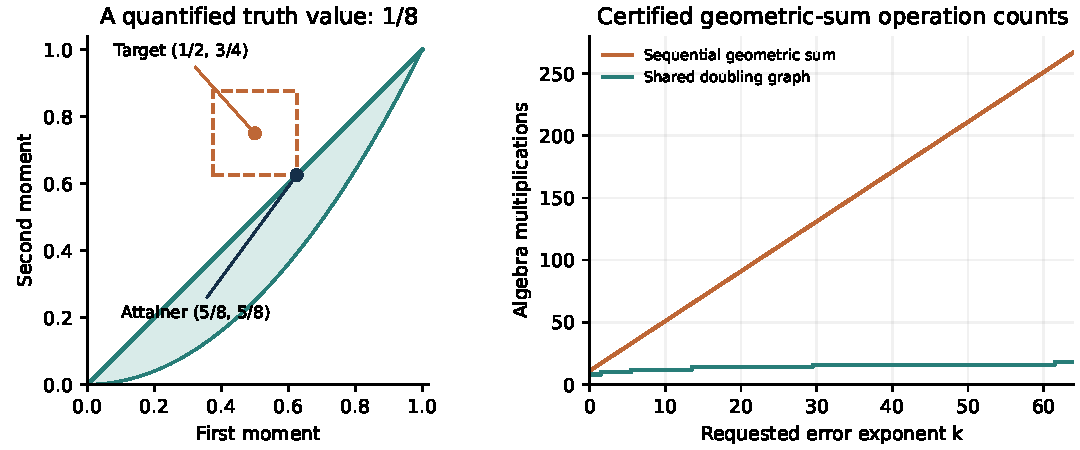
\includegraphics[width=\textwidth]{figures/observations.pdf}
\caption{Left: moment constraints make the continuous optimization problem
concrete. The smallest square centered at the target that meets the feasible
region has radius $1/8$. Right: algebra-operation counts for the explicit
Neumann clock $q=3/4$, $s=4$, $N=4(k+3)$, compared with its doubling evaluator.
These are exact operation counts for the prescribed algorithms, not elapsed-time
or bit-complexity benchmarks.}\label{fig:observations}
\end{figure}

\subsection{Formalization boundary and exact artifacts}

Define \code{AtomicLawCode} by a finite support array and rational weights
with Boolean nonnegativity and mass-one checks.  Define
\code{CouplingCode} by a rectangular rational array and its marginal
checks.  Implement \code{forestSolve}, \code{transport},
\code{pushRound}, and \code{probabilityNet} by the displayed bounded
algorithms.  Prove leaf-elimination preservation, cycle elimination,
finite gluing with the zero-marginal case, the rounding coupling, and
expectation stability in that order.  These are the additional finite
obligations before applying the already stated completion interface.
For object iPRA, each loop invariant consists of finite Boolean conditions,
cross-multiplied marginal equalities, and rational cost inequalities.
No unrestricted real quantifier is used as an induction matrix.

The checked Lean \code{argminQ_optimal} and
\code{finite_minimum_stability} kernels supply the finite quantifier
step.  The exact/supersolution budget theorem supplies shared error
propagation.  The transport and probability-net constructions themselves
are human proofs plus an implementation outline here, not completed Lean
theorems.  The accompanying \code{code/probability_models.py} uses exact
rational arithmetic to enumerate forests, check primal/dual certificates,
exercise gluing with a zero middle mass, construct a finite law net and
reproduce \eqref{eq:probability-moment-example}.  It records a denominator-8
three-center net with 45 valid laws and the exact attaining endpoint law.
These are finite implementation checks, not a substitute for the
object-theory derivations or a general construction of probability measures.

\section{Stable inverses and analytic functional calculus}\label{sec:analytic-algebras}

\subsection{A presented normed algebra}

Let $A_0$ be a unital associative algebra of finite codes over $\Q$, or over Gaussian rationals with central scalar action. Addition, subtraction, multiplication, and scalar operations are fixed PR programs. The algebraic laws have finite proofs. Norm bounds have finite rational certificates proving the triangle and submultiplicative inequalities; they may use the enclosure interface of Section~\ref{sec:completion}. Assume $\norm1\le1$. Write $\widehat A$ for the external norm completion, and retain only certified PR regular names when asserting an effective construction. Multiplication extends because, on bounded inputs,
\[
 \norm{ab-a'b'}\le\norm a\,\norm{b-b'}+\norm{a-a'}\,\norm{b'}.
\]
An input norm bound is obtained from its first name entry and its regularity bound, then enlarged rationally. Theorem~\ref{thm:extension} therefore supplies multiplication on the completion. Associativity and distributivity follow from the finite identities and arbitrarily small rational error. Scalar compatibility $\norm{ca}\le |c|\norm a$ is also part of the interface, where $|c|$ is the standard scalar modulus or a proved rational upper bound for it. For complex semantic conclusions the scalar action is central and extends continuously to complex scalars. This construction does not require local compactness or finite dimension.

All of the following identities are first proved for finite algebra expressions. Whenever the completion is mentioned, its use is justified by an explicit Cauchy estimate. In a semantic Banach algebra the same arguments have their familiar norm interpretation. In the arithmetic reading, every displayed norm inequality stands for its finite approximation contract.

\subsection{Finite geometric sums produce actual inverses}

For $R\in\widehat A$ write $S_N(R)=\sum_{j<N}R^j$, including $S_0=0$. The norm gap will always be supplied as
\begin{equation}\label{eq:neumann-gap}
 \norm R\le q=1-1/s,\qquad s\in\N,\quad s\ge1.
\end{equation}
Any rational upper bound strictly below one can be weakened to this form by choosing $s\ge1/(1-q)$ with a bounded integer ceiling.

\begin{lemma}[Finite Neumann identities and tail]\label{lem:neumann-finite}
For all $N$,
\[
 (1-R)S_N(R)=S_N(R)(1-R)=1-R^N.
\]
Under \eqref{eq:neumann-gap}, for $M\ge N$,
\begin{equation}\label{eq:neumann-tail}
 \norm{S_M(R)-S_N(R)}\le s q^N,
 \qquad q^{st}\le2^{-t}.
\end{equation}
\end{lemma}
\begin{proof}
Expanding either product telescopes the finite powers; equivalently, induct on $N$. No commutativity between arbitrary algebra elements is used. The tail norm is at most $\sum_{j=N}^{M-1}q^j$. The finite scalar identity
$(1-q)\sum_{j=N}^{M-1}q^j=q^N-q^M\le q^N$
gives the first bound. For the second, induction on $m$ proves $q^m(1+m/s)\le1$: the step uses
$q(1+(m+1)/s)\le1+m/s$.
At $m=s$ this says $q^s\le1/2$; another finite induction gives the result. This also covers $s=1,q=0$, with the usual convention $q^0=1$.
\end{proof}

Choose $H$ with $s\le2^H$. Then $N(k)=s(k+H+1)$ makes the tail at most $2^{-k-1}$. The families $S_{N(k)}$ are coherent by \eqref{eq:neumann-tail}; completing them gives $S(R)$. The identities of the lemma and $q^{N(k)}\to0$ give
\[
 (1-R)S(R)=S(R)(1-R)=1,\qquad \norm{S(R)}\le s.
\]
Thus invertibility has been constructed from a finite norm-gap certificate. It has not been inferred from an undecided spectral condition.

\begin{proposition}[Two residuals for a general approximate inverse]\label{prop:two-sided}
Suppose $A,B\in\widehat A$ and both
\[
 \norm{1-AB}\le q<1,\qquad \norm{1-BA}\le q<1
\]
have the gap certificate \eqref{eq:neumann-gap}. Then $A$ has inverse
\[
 X=B S(1-AB)=S(1-BA)B,
 \qquad \norm X\le s\norm B.
\]
The approximants $X_N=B S_N(1-AB)$ satisfy
\[
 AX_N=1-(1-AB)^N,\quad X_NA=1-(1-BA)^N,
 \quad\norm{X-X_N}\le s\norm B\,q^N.
\]
\end{proposition}
\begin{proof}
Put $R=1-AB$ and $L=1-BA$. The finite relation $BR=LB$ implies $BR^j=L^jB$ by induction, so the two finite formulas for $X_N$ agree. Applying the Neumann identities gives both residual equations. The tail bound gives a completed $X$, and both residuals tend to zero. Alternatively, the two series produce a right inverse $X_R$ and a left inverse $X_L$, which agree by $X_L=X_L(AX_R)=(X_LA)X_R=X_R$.
\end{proof}

\begin{remark}[A one-sided certificate is insufficient in infinite dimension]
Let $S(x_0,x_1,\ldots)=(0,x_0,x_1,\ldots)$ and $L(x_0,x_1,\ldots)=(x_1,x_2,\ldots)$ on $\ell^1$. Then $LS=I$, while $L$ has a nonzero kernel and $SL\ne I$. Taking $A=L,B=S$ gives zero right residual but no inverse. The two-sided hypothesis in Proposition~\ref{prop:two-sided} cannot silently be dropped when passing from square matrices to continuous operator algebras.
\end{remark}

For an already supplied inverse $B=A^{-1}$, a perturbation $E$ needs only the gap $\norm{BE}<1$, since
$A+E=A(1+BE)$ and the inverse is $S(-BE)B$. If $\norm B\norm E\le q=1-1/s$, the finite series proves
\[
 \norm{(A+E)^{-1}}\le s\norm B,\qquad
 \norm{(A+E)^{-1}-B}\le s\norm B^2\norm E.
\]
This is the quantitative form of openness of invertibility used below; no general spectral theorem is a premise.

\subsection{Fast geometric sums and named inputs}

Define
\begin{equation}\label{eq:doubling}
 P_0=R,\quad T_0=1,\qquad
 P_{j+1}=P_j^2,\quad T_{j+1}=T_j+P_jT_j.
\end{equation}
An induction proves
$P_j=R^{2^j}$ and $T_j=S_{2^j}(R)$, because the new summand contains exactly the powers from $2^j$ through $2^{j+1}-1$. There are two algebra multiplications per round. To reach a required term count $N\ge1$, choose the least $m$ with $2^m\ge N$ by a search bounded by $N$. This requires $2m$ multiplications rather than a linear number in $N$. The gain is in algebra operations; coefficient lengths and rational bit sizes must still be counted in an implementation-specific complexity analysis.

If multiplication is performed with finite numerical errors, treat the two recurrences as a shared graph and apply Section~\ref{sec:budgets}. Upper bounds for the ideal quantities are $\norm{P_j}\le1$ and $\norm{T_j}\le s$. With guards $\norm{P'_j}\le2$ and $\norm{T'_j}\le s+1$, one obtains the concrete propagation estimates
\[
 E_{P,j+1}\le3E_{P,j}+\delta_{P,j},\qquad
 E_{T,j+1}\le2E_{T,j}+(s+1)E_{P,j}+\delta_{T,j}.
\]
For the second identity, write the product discrepancy as
$P_j(T_j-T'_j)+(P_j-P'_j)T'_j$.
The error envelope and guard check are recorded together. Exact finite-code algebra, as in the reference examples, makes these operation errors zero.

An abstract named $R$ is handled without pretending that its exact value is a finite input. Let $r$ be a dense approximation with $\norm{R-r}\le\eta\le1/(2s)$. Then $\norm r\le1-1/(2s)$, so its finite polynomial evaluator has gap $2s$. The inverse identity
\[
 S(R)-S(r)=S(R)(R-r)S(r)
\]
gives error at most $2s^2\eta$. To meet target $\eps$, choose
\[
 \eta\le\min\{1/(2s),\eps/(4s^2)\},
\]
and make the finite-series tail for $r$ at most $\eps/2$. These choices are PR rational demands. The computed output is then within $\eps$ of $S(R)$; comparisons at two precisions prove regularity. If operations are rounded, divide the budget into three positive parts and use the graph certificate for the extra part. This explicitly separates input approximation, truncation, and arithmetic error.

\subsection{Power series in a noncommutative algebra}

Let $c_j$ be central scalar coefficients with a supplied majorant
\begin{equation}\label{eq:series-majorant}
 |c_j|R^j\le M\quad(j\ge0),\qquad R>0,\quad M\ge0.
\end{equation}
The coefficient evaluator is a fixed PR family, with a proof of this bound and a supplied approximation rate when its coefficients are named. Choose a rational radius $0\le r<R$ and restrict to $\norm a\le r$. Put $q=r/R$ and $f_N(a)=\sum_{j<N}c_ja^j$.

\begin{theorem}[Analytic evaluation with an explicit tail]\label{thm:analytic-evaluation}
The finite polynomials satisfy
\[
 \norm{f_K(a)-f_N(a)}\le\frac{M q^N}{1-q}\quad(K\ge N).
\]
They define a represented value $f(a)$ and, for $\norm a,\norm b\le r$,
\begin{equation}\label{eq:series-lipschitz}
 \norm{f(a)-f(b)}\le\frac{M}{R(1-r/R)^2}\norm{a-b}.
\end{equation}
Choose $s\ge1/(1-q)$ and $H$ with $Ms\le2^H$. The term count $N=s(k+H+1)$ makes the truncation error at most $2^{-k-1}$.
\end{theorem}
\begin{proof}
Submultiplicativity and \eqref{eq:series-majorant} bound each term by $Mq^j$. The finite geometric sum gives the tail and its clock. For stability, the noncommutative telescoping identity is
\[
 a^j-b^j=\sum_{i=0}^{j-1}a^{j-1-i}(a-b)b^i.
\]
Its norm is at most $jr^{j-1}\norm{a-b}$. Thus the finite-polynomial difference is bounded by
$\frac MR\sum_{j=1}^{N-1}j q^{j-1}\norm{a-b}$.
The sum is at most $(1-q)^{-2}$: its coefficients count pairs of nonnegative indices, so it is bounded by the product of two finite geometric sums, each at most $(1-q)^{-1}$. Pass to the coherent completion, or apply rational slack removal to finite approximants. This proves \eqref{eq:series-lipschitz}.
\end{proof}

Polynomial evaluation uses Horner's recurrence
$v_j=c_j+av_{j+1}$, starting from $v_N=0$. The usual backward induction gives $v_0=f_N(a)$, using $N$ multiplications. The large powers do not need to be separately constructed. Centrality of the coefficients guarantees agreement with the displayed power-series convention.

For named coefficients, first choose a rational guard radius $r<r'<R$ and compute the truncation clock of Theorem~\ref{thm:analytic-evaluation} using $r'$ in place of $r$. Approximate all $c_j$, $j<N$, at a precision for which
\[
 \e_p\sum_{j<N}r'^j\le\eps/4,
\]
The finite sum has the PR upper bound $N\max(1,r')^{N-1}$ when $N\ge1$. Choose the dense approximation $a'$ within $(r'-r)$ and also sufficiently close for \eqref{eq:series-lipschitz} at radius $r'$. Allocate the remaining budget to the geometric tail and, if needed, Horner-rounding errors. This gives a completely specified finite evaluator from fixed coefficient and input names. It requires no uniform evaluator for arbitrary analytic functions.

\subsection{A genuine derivative, including the noncommutative case}

The expression $f'(a)h$ is generally wrong in a noncommutative algebra. The correct derivative keeps the insertion position of $h$.

\begin{theorem}[Derivative and quadratic remainder]\label{thm:noncomm-derivative}
Under \eqref{eq:series-majorant}, for $\norm a\le r<R$, define
\[
 Df(a)[h]=\sum_{j\ge1}c_j
                  \sum_{i=0}^{j-1}a^iha^{j-1-i}.
\]
This is a bounded linear map with
\[
 \norm{Df(a)[h]}\le\frac{M}{R(1-r/R)^2}\norm h.
\]
If $\norm h\le t$ and $r+t<R$, then
\begin{equation}\label{eq:quadratic-remainder}
 \norm{f(a+h)-f(a)-Df(a)[h]}
 \le\frac{M}{R^2(1-(r+t)/R)^3}\norm h^2.
\end{equation}
The derivative series has a PR geometric tail on every supplied smaller radius, and therefore has a finite evaluator of the same kind as $f$.
\end{theorem}
\begin{proof}
The linear term at degree $j$ has $j$ summands and norm at most $jMr^{j-1}R^{-j}\norm h$. The same finite double-geometric bound used in Theorem~\ref{thm:analytic-evaluation} proves boundedness. Finite partial derivatives are linear; their uniform tail transfers linearity to the completion.

Expand $(a+h)^j$ as the sum of all ordered words in $a,h$. The words containing no $h$ give $a^j$, and the words containing one $h$ give precisely the displayed derivative. For each $\ell\ge2$, there are $\binom j\ell$ words containing $\ell$ copies of $h$. Their total norm is bounded by
\[
 \sum_{\ell=2}^j\binom j\ell r^{j-\ell}\norm h^\ell
 \le\binom j2(r+t)^{j-2}\norm h^2.
\]
The inequality follows coefficientwise from
$\binom j\ell\le\binom j2\binom{j-2}{\ell-2}$, since the right coefficient is $\binom\ell2\binom j\ell$. Sum over $j$. The coefficients $\binom j2$ count triples of nonnegative indices with sum $j-2$, so three finite geometric sums bound the result by the constant in \eqref{eq:quadratic-remainder}. The estimates apply first to finite tails and then to the completed values.

For an explicit derivative tail, select $r<r'<R$. For $j\ge1$,
\[
 jMr^{j-1}R^{-j}
 \le C(r'/R)^j,\qquad
 C=\frac{Mr'}{(r'-r)^2},
\]
because $j(r/r')^{j-1}\le(1-r/r')^{-2}$. Thus the derivative tail after degree $N-1$, for $N\ge1$, is at most
$C(r'/R)^N/(1-r'/R)\cdot\norm h$.
The block clock of Lemma~\ref{lem:neumann-finite} makes this a PR modulus. Fixing $r'$ also makes the remainder constant uniform for $\norm h\le r'-r$, which is exactly the Frechet differentiability assertion.
\end{proof}

An explicit differentiability demand is available as well. Fix $r<r'<R$, set $C=M/[R^2(1-r'/R)^3]$, and choose
\[
 \delta(\eps)=\min\{r'-r,\eps/(1+C)\}.
\]
For $\norm h\le\delta(\eps)$, the remainder is at most $\eps\norm h$. This formula also handles $M=0$ without division by zero.

Over a complex Banach algebra the derivative is complex linear; over the reals it is real linear. For scalar complex inputs this is holomorphicity on the certified disk. For operator inputs it is an analytic map on the norm ball in the usual semantic reading. The finite arithmetic result consists of the series evaluator, derivative evaluator, and displayed remainder demand. No commutation of $a$ with $h$ has been assumed. These formulas supply a useful common interface for analytic operators, not only for scalar special functions.

\subsection{Multiplication of analytic expressions}

Suppose two series have coefficient bounds $|c_j|R^j\le M_f$ and $|d_j|R^j\le M_g$. Their convolution coefficients
$e_n=\sum_{j=0}^n c_jd_{n-j}$ satisfy
\[
 |e_n|R^n\le(n+1)M_fM_g.
\]
Choose $r<R'<R$. Then
\[
 |e_n|(R')^n\le\frac{M_fM_g}{(1-R'/R)^2},
\]
using the double-geometric estimate. Hence the product series has the same usable majorant form at radius $R'$.

\begin{proposition}[Local functional-calculus product law]\label{prop:product-calculus}
For $\norm a\le r<R'$, evaluation of the convolution series equals $f(a)g(a)$.
\end{proposition}
\begin{proof}
For finite polynomials, distribute the product and group the pairs of indices by their sum. Central coefficients and $a^ia^j=a^{i+j}$ give the convolution identity. The omitted pairs with $i+j\ge N$ have total norm at most
\[
 M_fM_g\sum_{n\ge N}(n+1)(r/R)^n.
\]
Every finite part of this tail is bounded by the geometric majorant at radius $R'$ just obtained, and so has a PR vanishing bound. The two rectangular partial sums also approximate $f(a)g(a)$ by the product stability inequality. Compare the two finite expressions and let the certified errors decrease. No rearrangement of an unconditionally unspecified infinite series is used.
\end{proof}

This is a local power-series functional calculus. It does not assert general holomorphic functional calculus around an arbitrary spectrum, spectral mapping, or a spectral-radius algorithm. Those results would require extra contour, resolvent, and domain certificates. Here the radius gap is explicit and every relevant infinite operation has an actual tail modulus.

\subsection{An infinite-dimensional worked example}

Let $A_0$ be finite rational sequences, with convolution product and norm
$\norm a_1=\sum_j|a_j|$. The unit is $(1,0,\ldots)$. Finite double-sum arithmetic proves $\norm{ab}_1\le\norm a_1\norm b_1$. Its completion is the presented part of $\ell^1(\N)$; a name includes a PR finite-support approximation rate. Interpreting a sequence as coefficients gives an absolutely convergent power series on the closed unit disk, since
\[
 \left|\sum_j a_jz^j\right|\le\sum_j|a_j|\quad(|z|\le1).
\]
Thus coefficient-$\ell^1$ error controls uniform complex function error.

Take
\[
 b(z)=z/4+z^2/8,\qquad\norm b_1=3/8.
\]
The geometric construction produces the function
\[
 u(z)=\frac1{1-z/4-z^2/8}
\]
as one coherent $\ell^1$ name, uniformly on $|z|\le1$. Its coefficients are determined by the fixed PR recurrence
$u_0=1$, $u_1=1/4$, and
$u_n=u_{n-1}/4+u_{n-2}/8$ for $n\ge2$.
Because the coefficients are nonnegative, the exact norm of the geometric-series tail after $N$ powers of $b$ is
\[
 \frac{(3/8)^N}{1-3/8}=\frac85(3/8)^N.
\]
The reference program compares the recurrence coefficients with finite convolution sums, checks the polynomial residual identity, and checks the doubling construction in exact rational arithmetic. It also demonstrates matrix inversion from two residuals and the noncommutative derivative formula with a genuine quadratic remainder. These tests validate selected implementations and constants; the universal assertions are the proofs above.

The example is more than a scalar computation. The same inverse element acts by convolution as a bounded operator on $\ell^1$, and the same finite certificate controls that operator. It also supplies a contractible two-term complex with differential multiplication by $1-b$. This links complex analytic evaluation, normed algebra, and the homotopy construction of the next section through one shared approximation.

\section{Normed chain complexes: repairing homotopies from a finite defect}
\label{sec:chain-repair}

The useful categorical output in this section is an explicitly represented
inverse \emph{up to chain homotopy}.  It is obtained from a quantitative
certificate, without first constructing homology groups, selecting quotient
representatives, or deciding membership in an image.  The underlying
perturbation idea is classical; see Crainic~\cite{crainic2004}, especially
Sections~2.2--2.3 and~3.4.  What matters here is its organization into exact
finite identities, rational bounds, a primitive recursive precision schedule,
and a precisely delimited iPRA application.

The existing categorical material already distinguishes fixed presentations,
finite tables, and an external category of specified programs
\cite{repo-categories}.  We retain that distinction.  Its obstruction to
selecting representatives merely from a bound on the number of components
\cite{repo-obstacles} is not removed by the construction below.  Instead,
an explicit contracting operator supplies the missing witness in a stable
analytic situation.

\subsection{Data and meaning of the norm bounds}

Fix a finite band of degrees and a graded rational normed vector space
$C_0=\bigoplus_i(C_0)_i$.  Each summand may be infinite dimensional.
Valid core vectors, addition, rational scalar multiplication, and a rational
norm are given by fixed PR recipes.  Their algebraic and norm laws are
supplied with the arithmetic proofs required by the framework.  Write
$\widehat C$ for the space of represented Cauchy names over this core.
This notation is external shorthand for the represented objects; it does
not quantify in iPRA over all sequences or over all real vectors.

A differential is a fixed linear recipe $D$ of degree $-1$, satisfying
$D^2x=0$ and $\|Dx\|\le B_D\|x\|$ on valid core vectors.  A candidate
contracting homotopy is a fixed linear recipe $h$ of degree $+1$, with
$\|hx\|\le H\|x\|$.  At the ends of the degree band the unavailable
components are zero.  The bounds extend these maps to represented
completions.  Throughout this section, notation such as $\|T\|\le b$
means the supplied assertion
\[
                         \|Tx\|\le b\|x\|
                         \quad\hbox{for every valid }x.
\]
It does not require computing an operator norm as an unbounded supremum.
Only the fixed recipes that occur in the proof are used.

The core-preserving case gives a direct PR construction.  The same finite
proof applies to represented operators that take core points to Cauchy
names when their finite compositions are supplied with evaluation and error
contracts.  In that version the error ledger must pay for those evaluations;
the algebraic identities alone do not supply them.  In particular, arbitrary
bounded operators are not silently included in a uniform evaluation domain.

Define the degree-zero defect and its finite correction by
\begin{equation}
 R=I-Dh-hD,\qquad
 S_N=\sum_{j=0}^{N-1}R^j,\qquad h_N=hS_N,\qquad S_0=0.
 \label{eq:chain-defect}
\end{equation}
All products mean composition, with the rightmost operator applied first.
The candidate need not satisfy $h^2=0$, and $h$ need not commute with $R$.

\begin{lemma}[Exact finite correction]
\label{lem:finite-chain-correction}
For every natural number $N$,
\begin{equation}
 DR=RD,\qquad DS_N=S_ND,\qquad
                Dh_N+h_ND=I-R^N.
 \label{eq:chain-finite-identity}
\end{equation}
\end{lemma}
\begin{proof}
Expanding the first equation and using $D^2=0$ gives
\[
 DR=D-D^2h-DhD=D-DhD
    =D-DhD-hD^2=RD.
\]
Induction on $j$ gives $DR^j=R^jD$: the successor calculation is
$DR^{j+1}=(DR^j)R=R^jDR=R^{j+1}D$.
Adding these equations proves $DS_N=S_ND$.  The two finite telescoping
identities are
\[
 (I-R)S_N=I-R^N=S_N(I-R).
\]
They hold for $N=0$ because both sides are zero.  Adding $R^N$ to $S_N$
adds $R^N-R^{N+1}$ to either product, which proves the successor step.
Finally,
\[
 Dh_N+h_ND
   =DhS_N+hS_ND
   =(Dh+hD)S_N
   =(I-R)S_N=I-R^N.
\]
Every step is an equation of finite terms.  In particular, this proof does
not use convergence, commutativity of the operator algebra, or a side
condition on $h^2$.
\end{proof}

\subsection{A fully explicit correction schedule}

Assume a rational defect certificate
\begin{equation}
      0\le\rho\le 1-2^{-s},\qquad
      \|R\|\le\rho,\qquad H\le 2^c,
      \qquad s,c\in\mathbb N.
 \label{eq:chain-margin}
\end{equation}
The non-strict rational inequality contains a positive margin even when the
actual operator norm is unknown.  A bare assertion $\|R\|<1$ must first
provide such a usable margin before it can serve as a numerical contract.

For $M\ge N$, finite expansion gives
\begin{align}
 \|h_N\|&\le H\sum_{j<N}\rho^j
                  \le\frac{H}{1-\rho},\label{eq:chain-bound}\\
 \|h_M-h_N\|&\le H\sum_{j=N}^{M-1}\rho^j
                  \le\frac{H\rho^N}{1-\rho}.
                  \label{eq:chain-tail}
\end{align}
These are finite geometric-sum estimates.  For example,
$(1-\rho)\sum_{j<N}\rho^j=1-\rho^N\le1$; multiplication by the
positive denominator justifies the displayed rational bound.  Bounds for
products follow from applying the two operator inequalities successively
to an arbitrary vector.  Thus no supremum principle is hidden here.

Here is a schedule that uses no logarithm, exponential approximation,
or unbounded least search.  For $0\le a\le1$, induction on $m$ proves
\begin{equation}
                   (1-a)^m(1+ma)\le1.
 \label{eq:rational-geometric-block}
\end{equation}
Indeed,
$(1-a)(1+(m+1)a)=1+ma-(m+1)a^2\le1+ma$.
Taking $a=2^{-s}$ and $m=2^s$ gives
$\rho^{2^s}\le1/2$, hence
\[
                         \rho^{2^s t}\le2^{-t}.
\]
Consequently
\begin{equation}
                  N(n)=2^s(n+s+c+2)
                  \label{eq:chain-schedule}
\end{equation}
makes the right side of \eqref{eq:chain-tail} at most $2^{-n-2}$.
After denominators are cleared, the induction invariant in
\eqref{eq:rational-geometric-block} is a quantifier-free inequality of
PR integer terms.  This is an explicit use of quantifier-free induction,
rather than induction over a proposition about all completed vectors.

\begin{theorem}[Repair of a represented contracting homotopy]
\label{thm:chain-repair}
Under the stated presentation laws and \eqref{eq:chain-margin}, the recipes
$h_N$ define a represented bounded linear map $\mathcal H$ on
$\widehat C$ satisfying
\begin{equation}
 \|\mathcal H\|\le\frac{H}{1-\rho}\le2^{s+c},\qquad
 D\mathcal H+\mathcal H D=I,
 \label{eq:chain-repaired}
\end{equation}
and
\begin{equation}
          \|\mathcal H-h_N\|
                   \le\frac{H\rho^N}{1-\rho}.
          \label{eq:chain-limit-tail}
\end{equation}
The map and all its requested observations have fixed PR recipes.
\end{theorem}
\begin{proof}
For a fixed core vector $x$, the estimate \eqref{eq:chain-tail}, multiplied
by a supplied bound on $\|x\|$, gives a PR Cauchy modulus for $h_Nx$.
The completion construction therefore represents its limit.
There is also an explicit diagonal formula for a non-core input.
Suppose $x_m$ is the fixed PR name of $x$, with
$\|x-x_m\|\le2^{-m}$ and $\|x\|\le2^b$.  Set
\[
 m=n+s+c+3,\qquad
 N=2^s(n+b+s+c+3),\qquad y_n=h_Nx_m.
\]
The error from the input name is at most
$2^{s+c}2^{-m}=2^{-n-3}$.  The truncation error on $x$ is at most
$2^{s+c+b}\rho^N\le2^{-n-3}$.  Thus $y_n$ is a rational-core
observation of the desired output with error at most $2^{-n-2}$.
The use of $x_m$ is schematic over this fixed name program, not an
evaluation operation for arbitrary PR program codes.

Each $h_N$ is linear.  To prove linearity of the limit, put the finitely
many inputs in one ball, use the same sufficiently large cutoff for all
of them, and apply the linearity equation for that finite cutoff.  The
sum of the explicitly bounded tail errors tends to zero with the displayed
schedule.  Equality in the separated completion gives the desired
linearity equation.  The finite bound \eqref{eq:chain-bound} similarly
passes to the limit, and \eqref{eq:chain-tail} gives
\eqref{eq:chain-limit-tail}.

For clarity, the limiting identity can be checked without invoking an
abstract theorem about an operator space.  For every fixed $x$,
\begin{align*}
 \|(D\mathcal H+\mathcal H D-I)x\|
 &\le \|D(\mathcal H-h_N)x\|
       +\|(\mathcal H-h_N)Dx\|+\|R^Nx\|\\
 &\le \left(1+\frac{2B_DH}{1-\rho}\right)\rho^N\|x\|.
\end{align*}
The last expression is below any prescribed dyadic error by a PR
schedule obtained from \eqref{eq:rational-geometric-block} and a rational
upper bound for its constant factor.  Therefore its represented value is
zero.  This proves \eqref{eq:chain-repaired}.
\end{proof}

The proof produces a single output name by diagonalization.  It does not
assume that every pointwise Cauchy family of operators has a uniform
computable limit.  The uniform majorant \eqref{eq:chain-tail} is the
specific extra information that permits this construction.

\subsection{Only compute the boundary observation that is needed}

A cycle is a vector $x$ satisfying $Dx=0$; a boundary is a vector of
the form $Dy$.  Equation \eqref{eq:chain-repaired} supplies the boundary
witness $y=\mathcal Hx$ for every represented cycle.  No test for the
equality $Dx=0$ is required: the conclusion is conditional on that
equation, while the output recipe is defined for every input.

Often one needs only a boundary approximation.  The exact finite identity
already gives
\begin{equation}
 x-Dh_Nx=h_NDx+R^Nx,
 \qquad
 \|x-Dh_Nx\|
 \le\frac{H}{1-\rho}\|Dx\|+\rho^N\|x\|.
 \label{eq:approximate-cycle}
\end{equation}
This also controls an approximate cycle.  In particular, for $Dx=0$ and
$\|x\|\le2^b$, the shorter cutoff
\begin{equation}
                 N_{\rm boundary}(n,b)=2^s(n+b)
                 \label{eq:boundary-cutoff}
\end{equation}
guarantees $\|x-Dh_Nx\|\le2^{-n}$.  The convention $R^0=I$ makes
the case $n=b=0$ valid as well.  This contract concerns the exact finite
value $h_Nx$; any numerical approximation to it must pay its own input
and evaluation errors through the ledger.

The smaller cutoff does not claim that $h_Nx$ itself is already close to
the full homotopy value.  It is sufficient for the requested boundary
observation, whose error is the residual $R^Nx$.  This is a useful example
of why the observation to be exported should determine the computation.

\subsection{Stable neighborhoods of a certified differential}

Let $D'=D+\Delta$ have the same degree, and suppose the exact structural
equation $(D')^2=0$ is supplied.  Suppose also that
\[
           \|I-Dh-hD\|\le\rho_0,\qquad
           \|h\|\le H,\qquad \|\Delta\|\le\delta.
\]
The new defect is
\begin{equation}
 R'=I-D'h-hD'=R-\Delta h-h\Delta,
 \qquad \|R'\|\le\rho_0+2H\delta.
 \label{eq:chain-perturbation}
\end{equation}
Thus any supplied inequality
$\rho_0+2H\delta\le1-2^{-s}$ allows
Theorem~\ref{thm:chain-repair} to construct a corrected contraction
for $D'$.  The old candidate may itself be only approximate.  If it is
an exact contraction, take $\rho_0=0$.

For a family with a certified bound
$\|D_t-D_u\|\le L|t-u|$, this gives an explicit neighborhood of each
certified parameter: any radius $r$ satisfying
$\rho_0+2HLr\le1-2^{-s}$ works.  It does not provide a contraction
on an entire parameter path unless that path is covered by appropriate
certificates.  Also, a small value of $(D')^2$ cannot replace the equation
$(D')^2=0$: the commutation identity in
Lemma~\ref{lem:finite-chain-correction} uses that equation exactly.

\subsection{A categorical application through a mapping cone}

Let $(C,d_C)$ and $(E,d_E)$ be presented normed chain complexes, and let
$F:C\longrightarrow E$ be a represented bounded chain map, meaning
$d_EF=Fd_C$.  Its mapping cone is the graded direct sum
\[
 \operatorname{Cone}(F)_i=E_i\oplus C_{i-1},\qquad
 D_F=\begin{pmatrix}d_E&F\\0&-d_C\end{pmatrix}.
\]
Use the maximum norm on each direct sum.  The square of this block
operator is zero: its diagonal blocks are $d_E^2,d_C^2$, and its upper
right block is $d_EF-Fd_C$.  Hence this is again a valid differential.
Canonical inclusions and projections have norm at most one.

\begin{theorem}[A defect certificate gives a chain-homotopy inverse]
\label{thm:cone-homotopy-inverse}
Suppose a degree-$+1$ candidate $h$ on $\operatorname{Cone}(F)$ has
certified bounds $\|h\|\le2^c$ and
$\|I-D_Fh-hD_F\|\le1-2^{-s}$.
There is an explicitly represented bounded chain map
$G:E\longrightarrow C$ and explicit bounded homotopies witnessing
$FG\simeq I_E$ and $GF\simeq I_C$.
Their recipes and PR observation schedules are obtained from the one
correction construction above.
\end{theorem}
\begin{proof}
Repair $h$ and write the resulting degree-$+1$ contraction in blocks as
\[
                    \mathcal H=
                    \begin{pmatrix}A&B\\G&J\end{pmatrix}.
\]
Here $A$ and $J$ have degree $+1$, $G$ has degree zero, and $B$ has
degree $+2$, with the shifts determined by the cone.  The lower-left,
upper-left, and lower-right blocks of
$D_F\mathcal H+\mathcal H D_F=I$ are respectively
\begin{align*}
             -d_CG+Gd_E&=0,\\
               d_EA+Ad_E+FG&=I_E,\\
               GF-d_CJ-Jd_C&=I_C.
\end{align*}
The first equation says that $G$ is a chain map.  The second supplies
a homotopy from $I_E$ to $FG$; the third supplies a homotopy from $GF$
to $I_C$.  All three block maps have bounds at most
$2^{s+c}$, since the inclusions and projections have bound one.
Composing their fixed recipes with the output name of $\mathcal H$
gives the stated observation schedules.

At a finite cutoff the same block calculation has an error block of
$R^N$ on the right.  Each block has norm at most $\rho^N$.  Thus the
construction can also export finite approximate inverse and homotopy
equations without first materializing their limiting maps.
\end{proof}

For completeness, the categorical relation used here has an entirely
explicit presentation.  A prescribed homotopy from chain maps $f$ to $g$
is a degree-$+1$ map $K$ with $f-g=dK+Kd$.  The zero map witnesses
reflexivity, $-K$ reverses a homotopy, and addition composes two
homotopies.  If $u$ and $v$ are chain maps, then
\[
 u(f-g)=d(uK)+(uK)d,\qquad
 (f-g)v=d(Kv)+(Kv)d.
\]
Thus homotopy is a congruence for composition, and the theorem produces
an inverse arrow in the corresponding homotopy category.  This is a
scheme for fixed presented complexes and maps, not an internally coded
category containing every Banach space or every bounded operator.

The certificate is stable under simultaneous perturbations of both
complexes and of the map.  Write their changes as
$\Delta_C,\Delta_E,\Delta_F$, with bounds
$\delta_C,\delta_E,\delta_F$.  Assume the new differentials square to
zero and the new map is a chain map.  The cone differential changes by
\[
 \Delta_{\rm cone}=
   \begin{pmatrix}\Delta_E&\Delta_F\\0&-\Delta_C\end{pmatrix},
 \qquad
 \|\Delta_{\rm cone}\|
       \le\max(\delta_E+\delta_F,\delta_C).
\]
Substitution in \eqref{eq:chain-perturbation} gives a single rational
margin test for the perturbed chain-homotopy equivalence.  This preserves
the actual witness and its computational bound, rather than appealing to
an unspecified invariance theorem for homology groups.

\subsection{Continuous logic and the indispensable margin}

There is a direct connection to the continuous-predicate viewpoint
\cite{bbhu2008}.  For fixed $D,h$, the bounded predicate
\[
 x\longmapsto\min\{1,\|x-Dhx-hDx\|\}
                     \quad (\|x\|\le1)
\]
has a continuity modulus obtained from the bounds on $D$ and $h$.
A certified upper bound $\rho<1$ for this predicate on the whole unit
ball is exactly the sort of positive margin used by the correction
theorem.  On a represented finite dimensional compact ball, finite nets
and an explicit modulus can supply such a universal bound from finitely
many observations, including their discretization error.  For rational
matrices with the $\ell^1$ norm, one can instead compute the bound
exactly as the maximum absolute column sum.

An infinite dimensional Banach unit ball is not assumed to have finite
nets.  In that setting the universal bound must come from an operator
estimate or another supplied proof.  Neither this application nor the
existing fixed-formula continuous semantics supplies general compactness,
arbitrary model existence, or a finite net for every bounded metric sort.

The need for a margin is already visible in the two-term complex
\[
             0\longrightarrow\mathbb R
                   \xrightarrow{\;t\;}\mathbb R
                       \longrightarrow0.
\]
For a positive rational $t$, division by $t$ gives a contraction; a
certificate $t\ge2^{-a}$ bounds it by $2^a$.  At $t=0$, the
differential is zero and the contraction equation would say $0=I$.
Moreover, a contraction of norm at most $M$ for positive $t$ must satisfy
$1\le tM$.  Thus no uniformly bounded family of contractions can
extend through $t=0$.  The framework resolves the stable case and
exposes this genuine boundary; a different encoding does not eliminate it.

\subsection{Exact arithmetic and Lean obligations}

For rational finite matrices, all core calculations above are bounded
loops over rational entries, with norm bounds from finite sums and maxima.
For a fixed infinite core presentation, the required linearity, norm, and
differential laws remain explicit hypotheses until their iPRA proofs are
provided.  The finite induction lemmas concern equality or rational
inequality of encoded terms.  The completed-space theorem is assembled
from those finite contracts at each requested observation.  It is not
obtained by applying iPRA induction to a statement quantifying over all
Cauchy names.

One can make the finite invariant especially concrete.  Fix a core vector
$x$ and carry the four states
\[
 u_j=R^jx,\quad v_j=R^jDx,\quad
 \sigma_j=\sum_{i<j}R^ix,\quad
 \tau_j=\sum_{i<j}R^iDx.
\]
They are updated by $u_{j+1}=Ru_j$, $v_{j+1}=Rv_j$ and by adding
$u_j,v_j$ to the two sums.  The invariant includes
$Du_j=v_j$, $D\sigma_j=\tau_j$,
$(I-R)\sigma_j=x-u_j$, and the rational norm bounds on these finite
states.  Its step uses the supplied laws at the current core vectors.
This is a quantifier-free invariant with $x$ as a free parameter;
universal generalization over $x$ occurs after its induction proof.

An exact example uses degrees $0,1,1,2$ on four coordinates and
\[
 D=\begin{pmatrix}
 0&1&0&0\\0&0&0&0\\0&0&0&1\\0&0&0&0
 \end{pmatrix},\qquad
 h=\begin{pmatrix}
 0&0&0&0\\3/4&0&0&0\\1/16&0&0&0\\0&1/8&3/4&0
 \end{pmatrix}.
\]
In the $\ell^1$ norm, $\|h\|=13/16$ and
$R=\tfrac14 I-\tfrac{3}{16}\mathsf E_{32}$ has norm $7/16$,
where $\mathsf E_{32}$ is the matrix with its only nonzero entry in
row~3, column~2.  Here $h^2\ne0$ and $hR\ne Rh$.  Nevertheless the
correction gives the exact contraction
\[
 \mathcal H=\begin{pmatrix}
 0&0&0&0\\1&0&0&0\\1/12&0&0&0\\0&-1/12&1&0
 \end{pmatrix}.
\]
The margin parameters $s=1,c=0$ are valid without computing this
closed form.

The file \texttt{ObservableAnalysis/Neumann.lean} checks the exact
identities of Lemma~\ref{lem:finite-chain-correction} over a possibly
noncommutative ring.  Its definitions mirror the defect, geometric sum,
and corrected homotopy in \eqref{eq:chain-defect}.
The residual theorem is named
\texttt{correctedContraction\_residual}.
The remaining formalization steps are specific:
\begin{enumerate}
\item Realize core vectors and operators by the selected arithmetic
  presentation, and prove the degree, linearity, and norm contracts.
\item Prove the finite geometric inequality and the dyadic block estimate
  \eqref{eq:rational-geometric-block} with encoded rational arithmetic.
\item Apply the represented completion construction to the displayed
  diagonal name $y_n$, proving its error bound and extensionality.
\item Define the graded cone by finite tagged products, prove its
  square-zero identity, and extract the three block equations above.
\item Supply object-language iPRA proofs for the chosen presentation
  laws and finite induction instances.  The compiled Lean ring theorem
  is a verified algebraic metatheorem, not by itself an iPRA derivation.
\end{enumerate}

The exact-rational example in \texttt{code/check\_chain\_contraction.py}
uses a four-dimensional graded complex with $h^2\ne0$ and $hR\ne Rh$.
It checks the finite residual identities and compares the scheduled
approximants with an independently computed rational inverse.  The
recorded result in \texttt{evidence/chain\_contraction\_check.json}
is an example verification; the general finite identity is proved in the
Lean file and in Lemma~\ref{lem:finite-chain-correction}.

\section{Lean formalization: checked kernels and the completion path}\label{sec:formalization}

\subsection{What was actually compiled}

The archive contains a standalone project pinned to Lean 4.32.0. It uses only the distribution's standard library, with no Mathlib or ProveIt package dependency. Its five source files and all project source dependencies are enclosed. The captured build completed successfully. There are no \code{sorry}, \code{admit}, or new axiom declarations. This is useful evidence about the finite kernels; it is not evidence that the new analytic theorems have reached the embedded iPRA judgment.

\begin{longtable}{@{}P{.26\textwidth}P{.39\textwidth}P{.28\textwidth}@{}}
\toprule File & Checked result & Exact boundary\\\midrule\endhead
\path{ObservableAnalysis/Neumann.lean} & Left and right finite geometric identities; commutation with powers and sums; corrected-contraction residual. & An arbitrary supplied, possibly noncommutative ring. No normed-space convergence theorem is assumed or proved in this file.\\
\path{ObservableAnalysis/Budget.lean} & Finite sum laws and exchange; exact-balance and supersolution weighted-error implications for arbitrary finite size. & Ordinary Lean rational arithmetic and numerical hypotheses.\\
\path{ObservableAnalysis/FiniteMinimum.lean} & An explicit argmin on indices $0,\ldots,n$, its index bound and optimality, and uniform minimum stability. & A supplied finite rational table; no infinite infimum or compactness theorem.\\
\path{ObservableAnalysis/Blueprint.lean} & Typed PR syntax and metatheoretic evaluation; definitions of coding/presentation obligations; a proved bridge from budget records to the finite verifier. & Definitions with law fields are obligations, not implemented presentations or asserted correctness axioms.\\
\path{ObservableAnalysis.lean} & Imports the complete standalone project. & No additional mathematical claims.\\
\bottomrule
\end{longtable}

The algebraic residual theorem checks the actual expression
\[
 D\bigl(hS_N(1-Dh-hD)\bigr)
 +\bigl(hS_N(1-Dh-hD)\bigr)D
 =1-(1-Dh-hD)^N
\]
from $D^2=0$. It is not a restatement of the desired conclusion as a hypothesis. The budget verifier similarly proves the cancellation argument from the local inequalities and the independently supplied balance inequalities. These are substantial reusable kernels underlying the two main new constructions.

\subsection{The axiom audit is part of the result}

The Neumann identities and corrected-contraction theorem report dependencies on \code{propext} and \code{Quot.sound}; some elementary commutation lemmas use only \code{propext}. They do not depend on \code{Classical.choice}. The rational-budget, finite-sum, and minimum-optimality theorems additionally inherit \code{Classical.choice} through the standard \code{Rat} library. The exact reports are in \path{lean/build.log} and \path{lean/verification.json}.

Consequently, the host project is not advertised as an axiom-free or entirely constructive Lean development. This does not make its elementary inequalities false, but it does matter to the requested proof-theoretic endpoint. An eventual proof in object iPRA must be a proof value built from \code{PRAAx}; the host rational theorem is a guide and a checked mathematical kernel, not a substitute. Conversely, the use of classical tools in Lean's metatheory need not add axioms to an object derivation when the final proof value actually contains only the stated object rules. The distinction has to be established by the final type and dependency audit, not by descriptive terminology.

\subsection{Typed definitions supplied by the blueprint}

The main constructors and their meanings are as follows.

\begin{longtable}{@{}P{.28\textwidth}P{.65\textwidth}@{}}
\toprule Definition & Data and obligation\\\midrule\endhead
\code{PRCode n} & Arity-indexed syntax for zero, successor, projections, composition, and primitive recursion.\\
\code{PRCode.eval} & Its total host-Lean interpretation. This evaluator is explicitly not claimed to be PR uniformly in the syntax code and is never introduced as one iPRA symbol.\\
\code{RationalCodes} & Decoding and PR codes for arithmetic and comparison, together with required correctness propositions. No concrete instance is asserted in the blueprint.\\
\code{MetricData}, \code{MetricLaws} & Admissibility and rational distance recipes with nonnegativity, reflexivity, symmetry, and triangle obligations.\\
\code{Name}, \code{RegularName} & A fixed unary PR approximation recipe and the two-index regularity law of Section~\ref{sec:completion}. Parameter families use arity $r+1$ with $r$ numerical parameters held fixed.\\
\code{EqualitySchedule} & A fixed PR schedule after which same-index observations are within a requested error. For regular names this is equivalent to the paper's cross-index relation.\\
\code{ModulatedMap} & A fixed map and modulus recipe with an admissibility and continuity obligation.\\
\code{FiniteNetData} & Nonempty finite-net size and point recipes, admissibility, and a bounded covering specification.\\
\code{SimpleData} & Finite cell count, rational weight and value recipes, finite integral and $L^1$ norm, and a nonnegative-weight predicate. Common-refinement laws are supplied by the measured presentation in Section~\ref{sec:measure}.\\
\code{MajorantTail} & Nonnegative terms and a PR schedule that bounds every finite tail of arbitrary length. No infinite summation is an internal primitive.\\
\code{ContinuousFormula} & Finite syntax for atoms, rational constants, basic continuous connectives, and infimum/supremum binders. A well-scoped interpretation and each atom's evaluator/modulus remain client obligations.\\
\code{BudgetCertificate} & Finite errors, coefficients, reverse weights and balance laws, with the already proved \code{BudgetCertificate.sound}.\\
\bottomrule
\end{longtable}

The paper places the recursion counter last in its mathematical PR notation; the Lean evaluator places it first. These are projection/permutation conventions, not different recursion principles. Similarly, the measure section's one-sided regularity convention is related to the symmetric convention by the explicit shift $s_k\mapsto s_{k+1}$.

For equality schedules, cross-index equality implies
$d(x_n,y_n)\le2\e_n\le\e_k$ whenever $n\ge k+1$. Conversely, given a correct schedule, compare any two fixed observations through a common index beyond the schedule at precision $j$. Regularity bounds the extra distances; as $j$ increases their rational slack vanishes. Lemma~\ref{lem:slack} yields the cross-index relation. This proves the compatibility of the two definitions without a real-equality decision procedure.

\subsection{Exact finite targets for the main mathematical lemmas}

The following is a dependency-ordered implementation plan. Each target has all its numerical hypotheses specified earlier; the point here is to identify its actual induction matrix and the existing kernel it can reuse.

\paragraph{1. Rational coding and bounded reflection.}
Implement signed numerator pairs and positive denominators using ProveIt's existing PR language. Prove cross-multiplication correctness for addition, multiplication, comparison, absolute value, min/max, and bounded sums. Reuse \code{BoundedSyntax.program_correct} and its reflection theorem for fixed bounded formula syntax~\cite{repo-interfaces}. Define graph validity, partition validity, and finite matrix inequalities as those Boolean formulas. The induction matrices are equations between accumulator terms, or their decidable guarded inequalities.

\paragraph{2. The reverse-weight producer and dual verifier.}
Code $L,b,W$ as lists of rationals. The reverse producer uses a frozen table and a decreasing index encoded as $n\dotminus(t+1)$. Its invariant says that all processed rows satisfy \eqref{eq:reverse-weight}; this is a bounded Boolean conjunction. The verifier's finite-sum target is exactly Theorem~\ref{thm:dual}, with all denominators cleared. The host proofs \code{weighted_budget} and \code{weighted_budget_supersolution} already identify the required finite sum lemmas and the final cancellation. Guard correctness remains a separate input derivation.

\paragraph{3. The completion and extension interface.}
Prove rational slack removal and the two-index triangle estimates. Define the completed distance as in Section~\ref{sec:completion}. Construct the explicit shifted output code for Theorem~\ref{thm:extension}; prove its regularity with two precision parameters free, and generalize afterward. The diagonal-completion case uses one fixed two-argument PR family. The output-code constructor is external syntax recursion on the fixed recipe; the arithmetic theorem quantifies over numerical inputs, never over an internal universal evaluator.

\paragraph{4. Measured partitions and the Vitali bound.}
Give event codes, Boolean operations, finite measure, partition codes, and common-refinement code, with the precise laws in Section~\ref{sec:measure}. For each refinement, the invariant accumulates the original cell mass and the sum of its refined masses. The core analytic finite target is
\[
 \sum_iw_i|u_i-v_i|
 \le\sum_iw_iR_K(u_i)+\sum_iw_iR_K(v_i)
       +\delta\sum_iw_i+2K\sum_iw_i\mathbf1_{|u_i-v_i|>\delta}.
\]
All variables here are rational finite data; the only branching is a rational comparison. Add the two input-approximation estimates and the two tail-approximation estimates to obtain the $4\sigma$ term. Then use the completion interface. Domination by an $L^1$ majorant supplies the clipping tail but does not supply a rate of convergence in measure; keep that cutoff as an explicit additional theorem input.

\paragraph{5. Fubini and probability sorts.}
Prove the finite partial-integration contraction and instantiate \code{sumQ_exchange}. The contraction gives the output Cauchy bound without a new loss of precision. For the probability sort, implement forest enumeration, leaf elimination, rational coupling validation, and bounded minimization; its correctness proofs use only finite graph and sum invariants. The finite mass-rounding estimate then constructs actual net elements. Extend Lipschitz expectations to the represented transport completion before interpreting formulas. At a quantifier node, use the fixed formula's modulus and the checked finite-minimum stability theorem; apply external induction on the fixed formula syntax. No model-existence axiom is used.

\paragraph{6. Neumann, power series, and derivative evaluation.}
For a fixed coded algebra, prove the ring and norm laws on valid codes. Reify the exact identities in \code{Neumann.lean} into those operations. With $R^j$ and $S_j$ stored as one recursive state, the invariant records
$(1-R)S_j=1-R^j$ and the geometric norm bound. The finite tail assertion has three free numerical parameters: starting index $N$, tail length $m$, and requested accuracy $k$; its matrix bounds the corresponding finite sum. The block clock is proved by quantifier-free induction on the two geometric exponents. Horner and doubling use polynomial identities as loop invariants. For the derivative, use ordered words or the insertion-sum recurrence; the quadratic bound is a finite weighted sum of nonnegative terms. Only after these proofs are completed does the common completion interface introduce the semantic function and derivative.

\paragraph{7. Contracting homotopies and cone blocks.}
The exact finite algebra is already checked in \code{correctedContraction_residual}. Reify it for the fixed core recipes $D,h$ with $D^2=0$. The vector-state invariant given at the end of Section~\ref{sec:chain-repair} keeps the quantified core vector free during induction. Add the finite tail clock and the explicit input diagonal to obtain the map name. Tagged finite direct sums code the mapping cone; elementary block multiplication proves its square-zero law and extracts the three homotopy equations. No homology quotient construction or representative-selection procedure is required.

\subsection{How this joins the actual ProveIt proof calculus}

The intended endpoint is an actual derivation of a fully expanded formula, schematically
\[
 []\vdash[\mathrm{PRAAx}]\ 
 \forall\vec a\,\forall k\bigl(
   \operatorname{InputContract}(\vec a)\to
   \operatorname{OutputContract}(\vec a,k)\bigr).
\]
For a conditional presentation, unproved presentation laws remain explicit assumptions in the sequent; they must not be hidden in a claim of an unconditional theorem. For a concrete instance, substitute the already proved object derivations for those laws and discharge them by the existing composition rules. The final contract may include universally quantified precision comparisons, but no induction is applied to that whole formula.

The audited repository already supplies a typed realizer-graph frontend, bounded master verification, and object derivations for bounded-syntax compilation~\cite{repo-interfaces}. The new work should be added as providers and clients of those interfaces. It should not replace them with a second generic checker, nor label a host proposition \code{Prf} without constructing the required proof value. The proposed integration order is finite rational laws, weighted-budget verification, represented completion, measure and analytic providers, then the probability/model and homotopy clients.

\subsection{Reproduction and the role of executable examples}

From the package root, \code{python3 verify.py} runs the standard-library exact-arithmetic examples and writes a consolidated receipt. The examples cover the error-budget producer and verifier, moving spikes and Fubini, finite probability laws and moment optimization, convolution and noncommutative analytic evaluation, and the four-dimensional chain complex. Each report uses exact fractions for acceptance tests. Decimal summaries, when present, are display only.

For the Lean project, run \code{lake build} in \path{lean/} with the pinned toolchain. The project contains its own definitions and all local source dependencies. The future object-language integration uses the independently pinned ProveIt sources, which were inspected but are not necessary for the standalone build. The PDF is rebuilt with \code{python3 build_pdf.py} from the package root, or with \code{latexmk -pdf report.tex} from a correctly configured TeX environment using \path{paper/} as the working directory.

The example receipts are regression evidence. They do not certify universal mathematical statements, and the absence of a failed finite example would not close an unproved analytic or object-language obligation. The proof-status ledger records those distinctions claim by claim.

\section{Resolved difficulties, remaining boundaries, and integration}\label{sec:synthesis}

\subsection{What the framework now supplies}

The common interface is a finite numerical observation, a stability proof, and a stated semantic meaning. Its strength comes from sharing real mathematical work: a single completion theorem transports many stable operations; a single error verifier combines their budgets; a single geometric identity supports inverses, analytic evaluation, and homotopies; and a single finite integration calculus supports both $L^1$ convergence and continuous expectation predicates.

\begin{longtable}{@{}P{.25\textwidth}P{.37\textwidth}P{.31\textwidth}@{}}
\toprule Difficulty & Resolution proved in this report & Hypothesis retained\\\midrule\endhead
Repeated precision choices and duplicated subcomputations & Reverse sensitivity weights compute the least nonnegative linear certificate on a DAG; one shared value serves all consumers. & Proved local amplification and guard estimates.\\
A cyclic error system appears to require solving every coordinate & A dual supersolution bounds a requested observable directly. & The error inequality must already be proved; a valid supersolution is supplied or separately produced.\\
Independent simple-law approximations do not define joint operations & One Boolean event algebra provides coherent common refinements. & Concrete PR Boolean and finite-measure laws.\\
An unbounded integrable majorant seems to need an extra tail oracle & One simple approximant of the majorant produces a clipping threshold and tail bound. & Its supplied $L^1$ name; no pointwise modulus is extracted.\\
Pointwise arguments hide a convergence rate & A finite small-bad-set certificate plus clipping tails gives the explicit Vitali budget. & Quantitative convergence in measure or the displayed finite certificate.\\
Partial integration might depend on section representatives & A contractive map on rectangular simple functions extends to the $L^1$ completion and gives Fubini. & A supplied rectangular $L^1$ approximation family.\\
Quantified probability distributions seem to demand measure compactness & Explicit finite rational laws and weight rounding supply valid finite nets; expectation predicates extend continuously. & A compact metric presentation of the underlying space.\\
Formal power series are confused with convergent analytic values & A radius/majorant pair gives finite tails, Horner evaluation, a noncommutative derivative, and a quadratic remainder. & A positive radius gap and fixed coefficient evaluator.\\
An approximate inverse may be only one-sided & Two residuals construct a two-sided inverse; the unilateral-shift example proves why both matter. & Both norm gaps, or a previously certified inverse in a perturbation theorem.\\
Abstract homology quotients conceal witness selection & A finite contraction defect produces a bounded homotopy and, on a cone, a chain-homotopy inverse. & Exact square-zero/chain-map laws and a positive defect margin.\\
\bottomrule
\end{longtable}

These results resolve specific missing interfaces. They do not claim that every requested continuous theorem is now automatic. In particular, a fixed convergent coefficient presentation may be evaluated through the analytic algebra machinery, but discovering pole clearance, choosing compatible branches, or proving a Mellin--Barnes tail remains a separate problem. The earlier Meijer-$G$ packet explicitly identifies such guards and its uncompiled analytic scaffolds~\cite{repo-meijer}; this report provides reusable operations for their verified portions, not a retrospective proof of all of its claims.

\subsection{The model-theoretic scope is deliberately exact}

Infima and suprema of fixed continuous formulas on supplied finite-net presentations have numerical observations with explicit errors. This makes model theory useful as a language for approximation and transport~\cite{bbhu2008}. It does not make the exact predicate ``this real truth value is zero'' decidable, and it does not produce a model of an arbitrary consistent theory. The probability sort is built from valid laws with explicit transport nets; the operator examples instead use universal norm estimates on potentially noncompact balls. Conflating those two inputs would make the framework false.

Likewise, the category of specified represented objects and maps is external organizational language. Its identities, compositions, and witness-preserving operations are given by fixed numerical recipes with internal contracts. This does not introduce a universe of all categories, an unrestricted function type, arbitrary quotients, or a general axiom of choice into one-sorted arithmetic. The homotopy-category example is valuable precisely because it produces the inverse and its homotopies, rather than choosing representatives from an unspecified quotient.

\subsection{The limits that no error budget removes}

\begin{enumerate}
\item \textbf{No universal evaluation.} Lemma~\ref{lem:no-eval} excludes a total PR interpreter for every PR program. Fixed recipes, bounded tables, and a fixed finite primitive library remain legitimate.
\item \textbf{No automatic modulus extraction.} A true continuity or convergence statement need not arrive with the effective data required by these constructions. A proof of those data is part of the task, not a default assumption.
\item \textbf{No arbitrary branch or representative selection.} Finite solvability and bounds on the number of components do not themselves choose a coherent infinite object. The repository's categorical obstruction remains relevant~\cite{repo-obstacles}.
\item \textbf{No unrestricted dominated convergence claim.} The finite Vitali theorem uses a convergence-in-measure cutoff. The reverse-mathematical and metastable literature has other precisely stated inputs and conclusions~\cite{measureADR2012,measureADRMeta2012}; their higher-order recursion bounds cannot be silently identified with first-order PR functions.
\item \textbf{No global spectral or topological decision.} Failing a norm-gap certificate does not prove that an inverse or homotopy does not exist. Conversely, a local certificate proves only its stated neighborhood. Rank, image membership, and arbitrary spectral questions remain separate.
\item \textbf{No proof-status inflation.} Compiled host-Lean identities, exact numerical examples, human analytic arguments, and embedded-iPRA proof values are different deliverables. This package supplies the first three and a detailed path to the fourth for its new main analytic results.
\end{enumerate}

\subsection{A practical sequence for repository integration}

The repository already has the proof calculus and its foundational arithmetic. The next implementation should reuse it in the following order.

First, add the dual weighted-error theorem as an object derivation over coded rational arrays, together with its reverse DAG producer. This is a compact target whose complete host proof and quantifier-free invariant are supplied here. It can immediately simplify the precision accounting of several existing analytic packets.

Second, complete the shared represented-metric extension theorem with explicit error shifts and distance names. The measure, probability, analytic, and homotopy constructions then all reuse the same coherence and representation-independence proof. This reduces repeated proof work and makes the semantics of a completed value uniform across packets.

Third, add the measured-partition provider and finite Vitali estimate, then instantiate Fubini and the majorant-tail extraction. These modules supply new measure-theoretic content with small, transparent arithmetic proofs. In parallel, reify the noncommutative Neumann and contracting-homotopy identities for fixed coded algebras and linear cores; their universal algebraic Lean proofs are already available.

Finally, assemble the probability-sort continuous semantics, analytic functional-calculus evaluators, and mapping-cone clients. Each client should export its actual finite contracts and, where warranted, its all-precision completed meaning. A proof receipt should name the exact object formula, source commit, provider identities, kernel build, and axiom audit. This turns the report into concrete, reviewable implementation work while keeping the verified boundary explicit.

\subsection{Deliverable status}

The human arguments in this report are complete under their displayed quantitative presentation assumptions. The accompanying source and verification files record the exact arithmetic demonstrations, the compiled finite Lean kernels, and the remaining object-language steps. The source audit identifies the baseline so that this contribution can be compared with existing work without treating repeated background as a new theorem. The central improvement is a reusable path from a meaningful continuous observation to a small finite certificate, together with explicit constructions in areas where the prior packets lacked those providers.

\begin{thebibliography}{99}
\bibitem{repo}
V. Reshetnikov, \emph{ProveIt}, source snapshot
\texttt{b2341af5370cd8a43f72ebb2341c0d7d7395b634}, inspected 20 November 2026.
\href{https://github.com/VladimirReshetnikov/ProveIt/tree/b2341af5370cd8a43f72ebb2341c0d7d7395b634/Logic/PrimitiveRecursiveArithmetic}{PrimitiveRecursiveArithmetic directory}, especially its README, UNIFICATION-PLAN, ENDPOINTS, and Derivations index.
Immutable source paths and Git blob identities appear in \path{evidence/source_manifest.json}.

\bibitem{repo-recent}
\emph{ProveIt}, same snapshot. Research packets
\href{https://github.com/VladimirReshetnikov/ProveIt/tree/b2341af5370cd8a43f72ebb2341c0d7d7395b634/Logic/PrimitiveRecursiveArithmetic/docs/proofs/foundations/finite_observations_ipra_2026-11-20}{\emph{Finite observations of continuous mathematics}},
\href{https://github.com/VladimirReshetnikov/ProveIt/tree/b2341af5370cd8a43f72ebb2341c0d7d7395b634/Logic/PrimitiveRecursiveArithmetic/docs/proofs/foundations/ipra_abstract_analysis_2026-11-20}{\emph{Abstract and continuous mathematics through explicit presentations}},
\href{https://github.com/VladimirReshetnikov/ProveIt/tree/b2341af5370cd8a43f72ebb2341c0d7d7395b634/Logic/PrimitiveRecursiveArithmetic/docs/proofs/foundations/ipra_continuous_framework_2026-11-20}{\emph{Continuous mathematics in iPRA}},
\href{https://github.com/VladimirReshetnikov/ProveIt/tree/b2341af5370cd8a43f72ebb2341c0d7d7395b634/Logic/PrimitiveRecursiveArithmetic/docs/proofs/foundations/ipra_continuous_framework_2026-11-20_2}{\emph{From finite observations to continuous structures}}, and
\href{https://github.com/VladimirReshetnikov/ProveIt/tree/b2341af5370cd8a43f72ebb2341c0d7d7395b634/Logic/PrimitiveRecursiveArithmetic/docs/proofs/foundations/ipra_continuous_mathematics_2026-11-20}{\emph{Finite observations in constructive arithmetic}}.
Their READMEs were inspected; selected foundations, limits, and Hilbert-space sections were read in full.

\bibitem{repo-dag}
\emph{ProveIt}, same snapshot.
\href{https://github.com/VladimirReshetnikov/ProveIt/blob/b2341af5370cd8a43f72ebb2341c0d7d7395b634/Logic/PrimitiveRecursiveArithmetic/docs/proofs/foundations/ipra_cfp_contract_compiler_2026-11-15/paper/sections/04_contract_dag.tex}{Contract-DAG compiler} and
\href{https://github.com/VladimirReshetnikov/ProveIt/blob/b2341af5370cd8a43f72ebb2341c0d7d7395b634/Logic/PrimitiveRecursiveArithmetic/docs/proofs/foundations/ipra_cfp_contract_compiler_2026-11-15/paper/sections/06_precision.tex}{precision contracts and backward budgeting}; also the resources-and-elimination packet's predetermined demand-recursion construction.

\bibitem{repo-coupled}
\emph{ProveIt}, same snapshot.
\href{https://github.com/VladimirReshetnikov/ProveIt/blob/b2341af5370cd8a43f72ebb2341c0d7d7395b634/Logic/PrimitiveRecursiveArithmetic/docs/proofs/foundations/ipra_coupled_refinement_2026-11-19/paper/sections/03_coupled.tex}{Coupled rational actions: producing convergence and error bounds}, and its \emph{Exact boundaries and counterexamples} section.

\bibitem{repo-interfaces}
\emph{ProveIt}, same snapshot.
\href{https://github.com/VladimirReshetnikov/ProveIt/blob/b2341af5370cd8a43f72ebb2341c0d7d7395b634/Logic/PrimitiveRecursiveArithmetic/Derivations/Lean/IPRADerivations/Foundations/BoundedSyntax.lean}{\texttt{Foundations/BoundedSyntax.lean}},
\href{https://github.com/VladimirReshetnikov/ProveIt/blob/b2341af5370cd8a43f72ebb2341c0d7d7395b634/Logic/PrimitiveRecursiveArithmetic/Derivations/Lean/IPRADerivations/Foundations/RealizerGraph.lean}{\texttt{Foundations/RealizerGraph.lean}}, and
\href{https://github.com/VladimirReshetnikov/ProveIt/blob/b2341af5370cd8a43f72ebb2341c0d7d7395b634/Logic/PrimitiveRecursiveArithmetic/Derivations/Lean/IPRADerivations/Foundations/RealizerMasterInterface.lean}{\texttt{Foundations/RealizerMasterInterface.lean}}.
These source modules were inspected, not rebuilt in this task.

\bibitem{repo-categories}
\emph{ProveIt}, same snapshot.
\href{https://github.com/VladimirReshetnikov/ProveIt/blob/b2341af5370cd8a43f72ebb2341c0d7d7395b634/Logic/PrimitiveRecursiveArithmetic/docs/proofs/foundations/ipra_categorical_methods/paper/sections/04_categories.tex}{Categorical methods, Section 4}.
Git blob \texttt{c4690f44f0db27207a6595fcfe2f4ddb4d24e56a}.

\bibitem{repo-obstacles}
\emph{ProveIt}, same snapshot.
\href{https://github.com/VladimirReshetnikov/ProveIt/blob/b2341af5370cd8a43f72ebb2341c0d7d7395b634/Logic/PrimitiveRecursiveArithmetic/docs/proofs/foundations/ipra_categorical_methods/paper/sections/07_obstacles.tex}{Categorical methods, Section 7: obstacles}.
Git blob \texttt{f5e3fdd3302e54f0faec388bf0aae1981a784b36}.

\bibitem{repo-meijer}
\emph{ProveIt}, same snapshot.
\href{https://github.com/VladimirReshetnikov/ProveIt/blob/b2341af5370cd8a43f72ebb2341c0d7d7395b634/Logic/PrimitiveRecursiveArithmetic/docs/proofs/analysis/meijer_g_ipra_2026-11-16/README.md}{Meijer-$G$ iPRA packet README}, including its explicit analytic guards and formalization status.

\bibitem{oconnor2007}
R. O'Connor, \emph{A monadic, functional implementation of real numbers},
Mathematical Structures in Computer Science 17(1) (2007), 129--159.
\url{https://arxiv.org/abs/cs/0605058}.

\bibitem{spitters2006}
B. Spitters, \emph{Constructive algebraic integration theory without choice},
Dagstuhl Seminar Proceedings 05021 (2006), 1--13.
\url{https://doi.org/10.4230/DagSemProc.05021.9}.

\bibitem{crainic2004}
M. Crainic, \emph{On the perturbation lemma, and deformations},
arXiv:math/0403266 (2004), especially Sections 2.2--2.3, 3.4, and 3.8.
\url{https://arxiv.org/html/math/0403266v1}.

\bibitem{bbhu2008}
I. Ben Yaacov, A. Berenstein, C. W. Henson and A. Usvyatsov,
\emph{Model theory for metric structures}, in \emph{Model Theory with Applications to Algebra and Analysis}, vol. 2, LMS Lecture Note Series 350 (2008), 315--427.
\url{https://math.univ-lyon1.fr/~begnac/articles/mtfms.pdf}.

\bibitem{peyre2019}
G. Peyr\'e and M. Cuturi, \emph{Computational Optimal Transport},
Foundations and Trends in Machine Learning 11(5--6) (2019), 355--607.
\url{https://arxiv.org/abs/1803.00567}.

\bibitem{measurePZ2024}
I. Petrakis and M. Zeuner,
\emph{Pre-measure spaces and pre-integration spaces in predicative
Bishop--Cheng measure theory}, Logical Methods in Computer Science
20(4:2) (2024), 1--33.
\url{https://doi.org/10.46298/lmcs-20(4:2)2024}.

\bibitem{measureADR2012}
J. Avigad, E. T. Dean and J. Rute,
\emph{Algorithmic randomness, reverse mathematics, and the dominated
convergence theorem}, Annals of Pure and Applied Logic 163 (2012), 1854--1864.
\url{https://arxiv.org/abs/1106.0775}.

\bibitem{measureADRMeta2012}
J. Avigad, E. T. Dean and J. Rute,
\emph{A metastable dominated convergence theorem}, Journal of Logic and
Analysis 4:3 (2012), 1--19.
The arXiv version is titled \emph{Metastable convergence theorems}.
\url{https://doi.org/10.4115/jla.2012.4.3};
\url{https://arxiv.org/abs/1108.4400}.

\bibitem{repoExpectedValue}
V. Reshetnikov, \emph{ProveIt}, pinned commit \texttt{b2341af5370c},
\href{https://github.com/VladimirReshetnikov/ProveIt/blob/b2341af5370cd8a43f72ebb2341c0d7d7395b634/Logic/PrimitiveRecursiveArithmetic/docs/proofs/probability/expected_value_ipra_2026-11-16/paper/sections/10_effective_integration.tex}{\emph{Effective integration and continuous laws}}.
Source blob \texttt{465752843def}; full identifiers are recorded in the
source audit.

\bibitem{repoGridIntegral}
V. Reshetnikov, \emph{ProveIt}, same pinned commit,
\href{https://github.com/VladimirReshetnikov/ProveIt/blob/b2341af5370cd8a43f72ebb2341c0d7d7395b634/Logic/PrimitiveRecursiveArithmetic/Derivations/Lean/IPRADerivations/Analysis/GridIntegral.lean}{\texttt{Analysis/GridIntegral.lean}}.
Source blob \texttt{6487786ac131}; full identifiers are recorded in the
source audit.

\end{thebibliography}

\end{document}
